\documentclass[a4paper,12pt,twoside,BCOR=10mm]{scrbook}

% UoI MSc thesis template (English) V2.0.4 25.4.2022

% The license of this template is not fully clear, but: This template
% version is based on an earlier LaTeX template that was once available
% on a SENS UGLA page where the author and license are unknown.  As
% that version has obviously been put once online with the intend to be
% used by students, providing and using it should not be problem.

% Helmut Neukirchen https://uni.hi.is/helmut updated that earlier
% template using a tikzpicture-based approach for the title page
% created by Þór Arnar Curtis.

% The included logos are very likely copyrighted by the University of
% Iceland, but
% https://zeroheight.com/1b323cfd9/p/20f1e6-theses/b/29a61a
% states that the document is intended to make it easier for
% students, staff, and print-shops to format the thesis and ensure a
% standardised appearance. So providing them here and using them
% should be legal.


% Search below for "MODIFY THESE LINES ONLY": there you can enter your name, thesis title, etc.

% BibLaTeX is assumed for references. While Overleaf does this
% automatically for you, if you run it locally on the commandline,
% then you need to run first pdflatex MSc.tex, then biber MSc (without
% the .tex extension), and then again pdflatex MSc.tex


% Packages
\usepackage[utf8]{inputenc}
\usepackage[icelandic, english]{babel}
\usepackage{t1enc}
\usepackage{graphicx}
\usepackage[intoc]{nomencl}
\usepackage{enumerate,color}
\usepackage{url}
\usepackage[pdfborder={0 0 0}]{hyperref}
\BeforeTOCHead[toc]{\cleardoublepage\pdfbookmark{\contentsname}{toc}} % Add Table of Contents to PDF "bookmark" table of contents
\usepackage{appendix}
\usepackage{eso-pic}
\usepackage{amsmath}
\usepackage{amssymb}
\usepackage[sf,normalsize]{subfigure}
\usepackage[format=plain,labelformat=simple,labelsep=colon]{caption}
\usepackage{placeins}
\usepackage{tabularx}
\usepackage{enumitem}
\usepackage{listings}
\usepackage{xspace}
\usepackage{float}
\usepackage{caption}
% Packages used for title page layout
\usepackage{xcolor}
\usepackage{tikz}
\usepackage{arydshln}
\usetikzlibrary{positioning}
\pgfkeys{/pgf/number format/.cd,fixed,precision=2}

% https://tex.stackexchange.com/questions/374661/keyword-highlighting-not-working-in-python-with-listings
\lstdefinestyle{Python}{
    language        = Python,
    basicstyle      = \ttfamily,
    keywordstyle    = \color{blue},
    keywordstyle    = [2] \color{teal}, % just to check that it works
    stringstyle     = \color{green},
    commentstyle    = \color{red}\ttfamily
}

\def\averageWindSpeedLimit{20\xspace}
\def\nHiddenLayers{6\xspace}
\def\nPCA{10\xspace}
\def\nunits{256\xspace}
\def\nepochs{200\xspace}
\def\batchsize{128\xspace}
\def\penaltyRegularization{0.01\xspace}
\def\activation{relu\xspace}
\def\startDateVedur{2004\xspace}
\def\nVGHourly{120\xspace}
\def\nVedurHourly{231\xspace}
\def\nStationsWNails{152\xspace}
\def\nStationsCombined{318\xspace}
\def\nVedurMin{212\xspace}
\def\nVGMin{115\xspace}
\def\nStationsMin{327\xspace}
\def\berror{6.54}
\def\merror{4.78}
\def\baselineerror{\berror\xspace}
\def\modelerror{\merror\xspace}
\def\errorImprovement{\pgfmathparse{\berror - \merror}\pgfmathresult\xspace}
\def\perErrorImprovement{\pgfmathparse{(1-\merror / \berror)*100}\pgfmathresult\xspace}


% Blue color according to HÍ corporate design
\convertcolorspec{RGB}{16,9,159}{rgb}\tmphiblue
\definecolor{hiblue}{rgb}\tmphiblue


\setlength{\parskip}{\baselineskip}
\setlength{\parindent}{0cm}
\raggedbottom

\setkomafont{captionlabel}{\itshape}
\setkomafont{caption}{\itshape}
\setkomafont{section}{\FloatBarrier\Large}
\setcapwidth{\textwidth}
%\setcapwidth[l]{\textwidth} % The original template had the [l] which leads to a warning that it gets ignored, so to reduce warnings, removed it.
\setcapindent{1em}


\usepackage{lmodern} % Use Latin Modern (instead of the default Computer Modern that is rendered using a bitmap font).
\usepackage{fixcmex} % To fix that Latin Modern large symbol math fonts has by default only one size: https://tex.stackexchange.com/a/621536
% Times new roman font instead of the standard LaTeX fonts: has not been test -- try this on your own risk
%\usepackage[T1]{fontenc}
%\usepackage{mathptmx}


%%%%%%%%%%%%%%%%% Configurations (Useful defaults, but OK to change %%%%%%%%%%%%%%%%%%%
\graphicspath{{figs/}} % Figures in directory figs

% Bibliography

% \usepackage[sort&compress,authoryear]{natbib} % Uncoment if you want to used NatBib instead of BibLaTeX (and comment the bitlatex line below)

\usepackage{biblatex}  % BibLaTeX used for references. 
\usepackage{csquotes} % BibLaTex wants to have context sensitive quotes
\addbibresource{references.bib} %  Name of *.bib file containing references


%%%%%%%%%%% MODIFY THESE LINES ONLY %%%%%%%%%%%%%%%%%%%%%%%%%%%%%%%%%%%%%%%%%%%%%%%%%%%%%%%%%

% Some note on advisor(s) vs. thesis committee: At the School of
% Engineering and Natural Sciences, according to Regulation
% no. 994-2017
% https://english.hi.is/university_school_of_engineering_and_natural_sciences/regulation_no_994_2017_on_masters_study_at
% Article 5., a student has an administrative supervisor who is
% typically also the academic supervisor, i.e. supervising the thesis.
% If someone from outside is supervising, than the person becomes the
% academic supervisor and you have in addition the administrative
% supervisor from within HÍ.
% In addition, according to Article 7., there is a Master's degree
% committee that includes at least two persons, one of which shall be
% the student’s administrative supervisor.
% Despite these formally defined roles, it is somewhat a matter of
% taste whether you list all persons as supervisors or all as just
% thesis committee or list the one single academic supervisor as
% supervisor and then all persons (repeating the supervisor's name)
% as thesis committee.
% In the settings, that follow here, you can set this and many other settings.

\def\thesisyear{2024}       					% Year thesis submitted
\def\thesismonth{September}					% Month thesis submitted, e.g. "December"
\def\thesisauthor{Brynjar Geir Sigurðsson}				% Thesis authoreiningaraðferðinni
\def\thesistitle{A NN approach to predicting gust factors in complex landscape} % Title of thesis
%\def\thesissubtitle{XXSubtitle is rarely usedXX}		% Subtitle of thesis (optional)
\def\thesisshorttitle{} 	% Optional: if title of thesis is longer than 50 characters, it would not fit on the spine (kjölur) and in this case you, need to provide a short title here for the print shop. Otherwhise: make it empty
\def\thesiscredits{60} 						% Credits awarded for the project
\def\thesissubject{Mechanical Engineering}
\def\thesiskind{M.Sc.}					% E.g. M.Sc. or Ph.D. thesis
\def\thesiskindformal{CCMagister Scientiarum}			% E.g. Magister Scientiarum
\def\thesisschool{School of Engineering and {Natural Sciences}}		% School
\def\thesisfaculty{Industrial Engineering, Mechanical Engineering and Computer Science}% Faculty name without "Faculty of" (gets added) 
\def\thesisaddress{Dunhagi 5}			        % Faculty or school office address street
\def\thesispostalcode{107}			                % Faculty or school office zip code
\def\thesistelephone{525 4000}					% Office telephone
%\def\thesispublisher{XX}					% Publisher (not used)
\def\thesissupervisors{Kristján Jónasson}					% Names of supervisors (split by \\ if more than one).
\def\thesisnrofsupervisors{1}					% Number of supervisors (to use "Supervisor" vs. "Supervisors")
\def\thesiscommittee{Kristján Jónasson \\ Ólafur Pétur Pálsson}			% Thesis commitee must include the supervisor(s)
\def\thesisexaminer{XXNN3XX}				        % Examiner (prófdómari)
\def\thesisISBN{}           					% Thesis ISBN number (keep empty: not used anymore)
\def\thesisprinting{}						% Name of printsthop (keep empty if thesis is never printed)
%\def\thesisprinting{Háskólaprent, Fálkagata 2, 107 Reykjavík}	% Name of printsthop (keep empty if thesis is never printed)
\def\thesislicense{This thesis may not be copied in any form without author permission.} % Set license here (could also be some Creative Commons license)
%\def\thesiskeywords{Keyword1, Keyword2, Keyword3}		% Keywords (not used anywhere, hence commented out)

%%%%%%%%%%% STOP MODIFYING HERE %%%%%%%%%%%%%%%%%%%%%%%%%%%%%%%%%%%%%%%%%%%%%%%%%%%%%%%%%

%%%%%%%%%%% Next modifications: search for "START MODIFYING HERE AGAIN" below %%%%%%%%%%

% We need this command if someone used \\ in the thesis title
\newcommand{\removelinebreaks}[1]{%
  \begingroup\def\\{}#1\endgroup}

% To be able to use units in equations. From https://qerub.se/typesetting-units-in-latex
\newcommand{\unit}[1]{\ensuremath{\, \mathrm{#1}}}

\begin{document}
\hypersetup{pageanchor=false}
\pagenumbering{Alph} % To prevent page numer "1" to be used multiple times, used "A", "B", etc. for the first pages
\begin{titlepage} % This titlepage environment spans in fact multiple pages

% This must be placed after "\begin{document}":
\lstset{
    frame       = single,
    numbers     = left,
    showspaces  = false,
    showstringspaces    = false,
    captionpos  = t,
    caption     = \lstname
}

% This is the cover title page. If you go to a print shop, they will
% ignore it and create their own cover page, i.e. this cover page here
% is only used by the PDF version that gets electronically archived.

  \thispagestyle{empty}
  
  % The banner at top and bottom (using a tikz overlay)
  \begin{tikzpicture}[remember picture,overlay]
    \node[anchor=north west, inner sep=0pt] at (current page.north west)
        {
\includegraphics[width=\paperwidth]{banner}}; % The top banner (as a PNG) % TODO: A vector graphic would be better

    \node(bottom)[shape=rectangle, fill=hiblue, minimum height=10mm, minimum width=\paperwidth, anchor=south west] at (current page.south west) {}; % The bottom banner (a filled rectangle)

    \node[above=0.4cm of bottom] {
        \begin{tabular}{c} 
          \sffamily \small \textcolor{hiblue}{\textbf{\MakeUppercase{Faculty of \thesisfaculty{}}}}
        \end{tabular}
    };
  \end{tikzpicture}

  \enlargethispage{3cm}
  \vspace*{3.5cm} % Here starts the white space below the top banner
  
  % The centering used below is with respect to the page margins which
  % are not the same on left and right which prevents proper centering
  % with respect to the tikz centering (and the title page in
  % general).  Instead, we use a minipage that we shift horizontally
  % by 2.6 cm.  But minipage sets \parskip to 0, so we need to save
  % and restore it.  To be able to use vfill/stretch in a minipage,
  % the height needs to be specified: 20.0 cm.
  \newlength{\currentparskip}
  \setlength{\currentparskip}{\parskip}
  \hspace*{-2.6cm}
  \begin{minipage}[t][20.0cm]{1.0\paperwidth}
    \setlength{\parskip}{\currentparskip}
    \begin{center}
      \vspace*{ \stretch{1.5} }
      \huge \sffamily \bfseries \thesistitle{}
    
      %\normalfont \LARGE \sffamily \thesissubtitle{}

      \vspace{ \stretch{1.0} }
      \normalfont \Large \sffamily \thesisauthor{}

      \vspace*{ \stretch{2.75} }

      \thesismonth{}~\thesisyear{} % E.g. "March 2022"

      \vspace{ \stretch{0.5} }
    
      \normalfont \Large \sffamily {\thesiskind{}~thesis \\
      in \thesissubject{}}

      \vspace*{ \stretch{1.0} }
    \end{center}
  \end{minipage}

  \newpage

  \thispagestyle{empty} \mbox{} % This is the inside page of the cover (cover verso) which remains empty

  \newpage


  \thispagestyle{empty} % This is the inner title page
  \begin{center}
    \vspace*{ \stretch{0.5} }

    \Large \sffamily \bfseries \thesistitle{}
    
    %\normalfont \large \sffamily \thesissubtitle{}

    \vspace*{ \stretch{1.0} }

    \sffamily{\thesisauthor{}}
    
    \vspace*{ \stretch{1.0} }
    \normalsize \thesiscredits{}~ECTS thesis submitted in partial fulfillment of a \\
    \textit{\thesiskindformal{}} degree in \thesissubject{}
    \large
    
    \ifx\thesissupervisors\empty % Only print supervisor part if supervisor names are not empty
    \else
      \vspace*{ \stretch{1.0} }
      \ifnum\thesisnrofsupervisors>1 Supervisors \\
      \else Supervisor \\
      \fi
      \thesissupervisors{}
    \fi  

    \ifx\thesiscommittee\empty % Only print thesis committee part if committee names are not empty
    \else
      \vspace*{ \stretch{0.25} }
      \thesiskind{}~Committee\\
      \thesiscommittee{}
    \fi
      
    \ifx\thesisexaminer\empty % Only print examiner part if thesisexaminer is not empty
    \else
      \vspace*{ \stretch{0.25} }
      Examiner \\
      \thesisexaminer
    \fi
      
    \vspace*{ \stretch{1.0} }

    Faculty of \thesisfaculty \\
    \thesisschool \\
    University of Iceland \\
    Reykjavik, \thesismonth~\thesisyear

    \vspace*{ \stretch{0.5} }
  \end{center}

  \newpage

  \thispagestyle{empty} % This is the title verso (colophon), i.e. imprint/copyright page
  \vspace*{\fill}
  % \setcounter{page}{0} \renewcommand{\baselinestretch}{1.5}\normalsize
  \sffamily{\removelinebreaks{\thesistitle}} \\
  \ifx\thesisshorttitle\empty % Show only if shorttitle is provided
  \else
  (\sffamily{\thesisshorttitle{}}) \\
  \fi
  %\sffamily{\removelinebreaks{\thesissubtitle{}}} \\

    
  \thesiscredits ~ECTS thesis submitted in partial fulfillment of a \thesiskind{}~degree in \thesissubject
\\ \\
  Faculty of \thesisfaculty \\
  \thesisschool \\
  University of Iceland \\
  \thesisaddress \\ 
  \thesispostalcode, Reykjavik 
  Iceland

  Telephone: \thesistelephone \\ \\ 
  \vspace*{\lineskip}

  Bibliographic information: \\
  \thesisauthor{} (\thesisyear{}) \emph{\removelinebreaks{\thesistitle{}}}, \thesiskind{}~thesis, Faculty of \thesisfaculty, University of Iceland.\\

  Copyright \textcopyright~\thesisyear~ \thesisauthor \\
  \thesislicense{}\\

  \ifx\thesisISBN\empty % Show only if ISBN is provided
  \else
  ISBN~\thesisISBN
  \fi
  
  \ifx\thesisprinting\empty % Show only if print shop is provided
  \else
  Printing: \thesisprinting \\
  \fi


  Reykjavik, Iceland, \thesismonth~\thesisyear \\
  
%%%%%%%%%%% START MODIFYING HERE AGAIN %%%%%%%%%%%%%%%%%%%%%%%%%%%%%%%%%%%%%%%%%%%%%%%%%%%%%%%%%

  \newpage % Dedication page: remove completely if you have no dedication

  \thispagestyle{empty} \mbox{}

  \vfill

  \begin{center}
    \textit{
      To all the students who made the wise decision to use \LaTeX. % Replace this by your dedication
    }
  \end{center} \vspace*{5cm}

  \vfill 

%%%%%%%%%%%%%%%%%%%%%%%%% If you have no dedication: remove until here %%%%%%%%%%%%%%%%%%%%

\end{titlepage}

\cleardoublepage

\pagenumbering{roman} % Abstract page 

\setcounter{page}{5}

\setkomafont{section}{\huge} % The title "Abstract" and "Útfdráttur" should look like the chapters, i.e. use \huge (\chapter cannot be used as this would create a new page)
\section*{Abstract}
English abstract (ca. 250 words).

\vfill \vspace*{1cm}

\section*{Útdráttur}
Hér kemur útdráttur á íslensku sem er að hámarki 250 orð.
\vfill

\newpage % Empty page
\setkomafont{section}{\FloatBarrier\Large}
% The first "chapter" which will start on a new page
% Table of contents starts automatically on a right-hand side page ("recto").
% Table of contents, list of figures and tables are automatically generated by the commands below
\hypersetup{pageanchor=true}
\tableofcontents
\listoffigures
\listoftables
\lstlistoflistings

\chapter*{Abbreviations}
\addcontentsline{toc}{chapter}{Abbreviations}
\markboth{Abbreviations}{Abbreviations}

Í þessum kafla mega koma fram listar yfir skammstafanir og/eða breytuheiti. Gefið kaflanum nafn við hæfi, t.d.\ Skammstafanir eða Breytuheiti. Þessum kafla má sleppa ef hans er ekki þörf. \\

The section could be titled: Glossary, Variable Names, etc.

If you use acronyms, it is strongly recommended to use a LaTeX
acronyms package. For example, to use the package \emph{acronym}, add
in the preamble:
\begin{verbatim}
\usepackage{acronym}
\end{verbatim}
and then here in this chapter (to create the list of all acronyms), use:
\begin{verbatim}
\begin{acronym}[SENS]
  \acro{SENS}{School of Engineering and Natural Sciences}
  \acro{UoI}{University of Iceland}
\end{acronym}
\end{verbatim}
In the square bracket above, you need to put the longest acronym, so
that the list gets proper indentation based on the longest acronym.
Also note that you need to manually sort here that list.

Then, whereever you use the acronym in your text: \verb|\ac{UoI}|:
that will automatically expand the acronym at the first use, but use
only the short version after the first use.  (Use \verb|\acp| if need
the plural form. \verb|\acl| if you explicitly want to have the long
form only, \verb|\acf| if you explicitly want to have the full long
and short form, i.e.\ like first use of \verb|\ac|.)

Use \verb|\acresetall| to forget about earlier usage (=expansion) of
acronyms, e.g.\ if despite already used in Abstract or Introduction,
but you want to expand them later once again (starting from, e.g., in
Foundations chapter): add \verb|\acresetall| at start of Introduction
chapter (and maybe also again at start of Foundations chapter).

\chapter*{Acknowledgments}
\addcontentsline{toc}{chapter}{Acknowledgments}
Í þessum kafla koma fram þakkir til þeirra sem hafa styrkt rannsóknina með fjárframlögum, aðstöðu eða vinnu. t.d.\ styrktarsjóðir, fyrirtæki, leiðbeinendur, og aðrir aðilar sem hafa á einhvern hátt aðstoðað við gerð verkefnisins, þ.m.t.\ vinir og fjölskylda ef við á. Þakkir byrja á oddatölusíðu (hægri síðu).

\pagenumbering{arabic}
\setcounter{page}{1}

% Chapter 1

\chapter{Introduction} % Main chapter title

\label{Chapter1} % For referencing the chapter elsewhere, use \ref{Chapter1} 

%----------------------------------------------------------------------------------------

% Define some commands to keep the formatting separated from the content 
\newcommand{\keyword}[1]{\textbf{#1}}
\newcommand{\tabhead}[1]{\textbf{#1}}
\newcommand{\code}[1]{\texttt{#1}}
\newcommand{\file}[1]{\texttt{\bfseries#1}}
\newcommand{\option}[1]{\texttt{\itshape#1}}

%----------------------------------------------------------------------------------------
Wind gusts are brief increase in wind speed (lasting seconds) as compared to mean wind speed. The gust factor is defined as the peak gust divided by the mean wind speed over some defined time period. The peak wind gust is often defined as the highest 3 second rolling average measured wind speed over a period of 10 minutes, while the mean wind is the average of all measurements in the 10 minute intervalf. This thesis uses this definition. This varies, with the US using a 1 minute interval, leading to 14\% higher results \cite{why_wind_gusts}. The Navier Stokes Equation (\ref{eqn:navierstokes}) shows that the change of the wind, in time and space, is dependent upon the pressure gradient, the oscillating force of the earth (the Coriolis force), and frictional force.\cite{uncertainties_in_numerical_weather_predictions}
\begin{equation}
    \label{eqn:navierstokes}
    \frac{\delta \mathbf{V}}{\delta t} + \mathbf{V}\cdot\nabla\mathbf{V} = \underbrace{-\frac{1}{\rho}\nabla P}_{pressure} -\overbrace{ f\mathbf{k}x\mathbf{V}}^{oscillation} - g - \underbrace{\frac{\delta(u'\omega')}{\delta z} - \frac{\delta(v'\omega')}{\delta z}}_{resistance}
\end{equation}

Traditionally, numerical weather prediction (NWP) systems are used to forecast and analyze weather patterns\cite{medium_range_3d_weather_forecasting_NN}. These models describe the transition between discretized packages of atmospheric states using partial differential equations based on physical reality. These results are usually published every hour, or at courser time intervals for climate simulations. With increasing computer power and efficiency the trend is to output data more often\cite{GNP_vidtal}.They describe the state over the period and so do not necessarily grasp fluctuations well. These fluctuations would include fluctuations in the wind speed, wind gusts\cite{canNNBeatNWP}.

This thesis looks at how best to predict gust factor based on various factors, using several different data sources, including NWP and observations. Being able to accurately predict the wind gust is important as it is often the peak wind gusts that will cause failures in structures. A problem that will become increasingly prevalent in the near future\cite{nasa_extreme_weather}.

\section{Background}
The history of numerical weather predictions goes all the way back to the 1920's when Lewis Fry Richardson pioneered the field and tried to produce forecasts. The results were flawed due to noise in the calculations. ENIAC was built in 1945, it was a general purpose computer that was used, among other things, to make predictions. These predictions took 24 hours to make and were predicting 24 hours into the future. It was a proof of concept but not usable\cite{TheENIACForecastsARecreation}. In the 1950's, with the advent of computers the first operational forecasts emerged. In September of 1954, Rossby and his Stockholm based team produced the first real-time barotropic forecasts. The next year the Joint Numerical Weather Prediction Unit (JNWPU), based in Princeton New Jersey, released their first forecasts. These forecasts were for 36 hours at 400, 700 and 900 mb. The results were inferior to subjective human-based forecasts but showed that such forecasts were feasible and promoted further development in the area \cite{historyNWP}. The field of NWP has taken great strides since then following the development of computer power and efficiency.

In the last decade there has been another transformation in the field of weather prediction driven by artificial intelligence. Interest in AI has come in waves. Some progress is made, then interest dwindles. Interest in AI has been increasing steadily since 2010. Notable work that has driven this wave of interest include increase in computational abilities due to parallel processing in graphical processing units (GPU), convolutional neural networks (CNN), which allowed much faster processing of massive (image) datasets and the availability of large datasets online. It is to be noted that images are grid data with some number of channels. Using CNNs could work on any gridded data where there are some spatial features\cite{canNNBeatNWP}. Since 2018, there has been significant work done in the weather prediction field using AI. In 2018, Dueben and Bauer showed that you can build a NN that can outperform a simple persistence forecast and is competitive with very coarse-resolution atmosphere models of similar complexity for short lead times\cite{dueben2018}. Also in 2018, Scher created a deep convolutional neural network (CNN) to emulate a general circulation model (GCM, a numerical model representing the physical processes), training on the GCM which allows it to emulate the dynamics of the model and maintain stability for much longer than Dueben\cite{scher2018}. These two papers were more proof of concept rather than production ready models to replace NWP. They showed that models based on deep learning might, with further development, compete with standard models in the field.

In the last two years there have been even more developments with the emergence of Large AI Weather forecast Models (LWM). In 2024, Ling et al.\cite{SecondRevolution} tried to standardize the definition of LWM in meteorology and came up with 3 rules that need to be met to count as LWM.

\begin{enumerate}[label = Rule \arabic*:]
    \item Large Parameter Count. The number of parameters can vary wildly but a general range might be from tens of millions to billions of parameters
    \item Large Number of Predictands: predicting on different levels (such as pressure levels or height levels) and offering detailed information on the atmospheric vertical structure and surface conditions
    \item Scalability and downstream applicability. This might crystallize in predicting cyclones. Often, the teams responsible for creating these models try to show their applicability to predict cyclones when not trained specifically on cyclone data (e.g. \href{https://www.youtube.com/watch?v=PD1v5PCJs_o&ab_channel=GregBronevetsky}{GraphCast})\cite{SecondRevolution}. This is done to show the versatility of the models.
\end{enumerate}

Before 2022, LWM had been shown to be able to compete with traditional NWP for some specifc cases as well as making predictions quicker, after training. No model had shown that it could in any way completely replace the traditional systems. In early 2022, Pathak et al.\cite{FourCastNet} presented FourCastNet. FourCastNet uses an Adaptive Fourier Neural Operator model that leverages transfomer architecture rather than the popular convolutional model architechture. FourCastNet matches the performance of standard forecasting techniques at short lead times for large-scale variables and outperforms for smaller variables. It generates a week-long forecast in less than 2 seconds, orders of magnitude faster than standard physical methods\cite{FourCastNet}. In 2022, machine learning methods were presented that made predictions much faster than traditional NWP, after a one time training (or at least training that wouldn't have to be redone often). These were in some cases performing better than NWP. In 2023, Remi Lam and the GraphCast team at Google introduced GraphCast. This model was able to outperform the industry standard High Resolution Forecast (HRES) produced by the European Centre for Medium-Range Weather Forecasts (ECMWF). This model as the name suggests leverages graphing connections rather than traditional grid like data structure. The base data is given in latitude and longitude degrees at a resolution of 0.25 degrees. This means points are closer to each other at the poles. Using the graphing structure is supposed to help with bias incurred as a result of this\cite{GraphCast}.

There has been a lot of progress made over the last 6 years (since 2018) and especially in the last 2 years (since 2022)\cite{SecondRevolution}. The progression from machine learning methods being an interesting idea in the field of numerical weather predictions, to outperforming the standard NWP has been remarkably quick. Two years ago, machine learning methods were able to predict quickly and in some niche cases outperform traditional models. They were not generally competitive with standard weather models. Now they are competitive. It is worth noting that the training of these large models is based on data from traditional large weather models. It will be very interesting to watch what the next few years will have in store for the development of machine learning in weather predictions.

\section{Methodology and related work}
This study looks at data from three sources and an attempt is made to predict the gust factor in a given place in Iceland. It uses reanalysis data, along with elevation data to predict the gust factor. It looks at the data at the point of interest. It does not look at the data as a time series. This thesis aims to improve on the baseline model of always predicting the mean gust factor and show that some structure can be learned from reanalysis data about gusts. To do this a neural network was created. Any significant improvement on a base model, that always guesses the mean gust factor, would indicate that the final model has something to contribute.

In 2004, H. Ágústsson and H. Ólafsson\cite{mean_gust_HA_HO} looked at the variability of gust factor in complex landscapes. They looked at data from automatic weather stations that measure wind at 10 meters above ground. The data that was studied in 2004 comes from the same source as used in this thesis, but limits itself to a smaller section. They only looked at the years 1999-2001. They looked at three factors and how these three parameters effected the gust factor. These were $d_m, D, H$, that is direction of wind blowing off a mountain, distance to the mountain and the height of the mountain above the weather station. Their main results were that the gust factor is inversely correlated to the distance from a mountain and correlated to the height of the mountain. The study in 2004 looked at the effect of a dominant point upwind. It did not look at the effects of the landscape more broadly. In this study, landscape upwind is looked at.

\subsection{Neural networks}
To be able to capture the patterns in the data a neural network was constructed. A NN architechture was chosen as they are known to be able to capture patterns well in complex data and handle high parameter counts. This comes in handy when training on different types of data. It is also easy to construct different types of neural networks and see how they fit well with parts of the dataset. A NN uses a lot of matrix calculations to weight input parameters and predict an output. A NN has some number of layers, a deep neural network (DNN) has an input layer, output layer and some number of hidden layers. Hidden layers are middle layers that take data from input layer and eventually reach the output layer. The input layer has a width equal to the number of parameters and the ouput has width equal to the number of predictants. Models were created for several number of parameters as a way to gauge the influence of each parameter. Each model has one numerical output variable. Each layer also has an activation function. There are several popular activation functions such as Rectified Linear Unit (ReLU), Exponential Linear Unit (ELU) and Hyperbolic tangetn (tanh). The definitions of ReLU, ELU and tanh can be seen in Equations (\ref{eqn:relu}), (\ref{eqn:elu}) and (\ref{eqn:tanh}). 

\begin{equation}
    \label{eqn:relu}
    r(x):=max(0, x)
\end{equation}

\begin{align}
    \label{eqn:elu}
    f(x) := x, x > 0\\
    f(x) := \alpha (e^x-1), x\leq 0, \alpha > 0
\end{align}

\begin{equation}
    \label{eqn:tanh}
    tanh(x):=\frac{e^x-e^{-x}}{e^x+e^{-x}}
\end{equation}

These activation control neural activation and can help stabilize the network.

\subsection{Model evaluation}
 To measure the performance of these models, both to train and test, mean absolute percentage error (MAPE) as defined in Equation (\ref{eqn:mape}) was used.
\begin{equation}
    \label{eqn:mape}
    \text{MAPE} = \frac{1}{n}\Sigma_{i=1}^n\frac{|y_{predict} - y_{true}|}{y_{predict}}
\end{equation}
This was chosen because the target is the gust factor (the wind gust over the average wind). If the target would have been the wind gust rather than the gust factor then something like mean absolute error might be more appropriate.

\subsection{Model explainability}
Neural networks are often considered as mysterious black boxes\cite{nn_black_box}. In an attempt to understand the model predictions, methods designed for explainability are used. One such method is Shapley values\cite{shapley_information}. Shapley values are calculated as the average marginal contribution of a feature value across all possible coalitions. For any combination of parameters what is the contribution of a given parameter. This means that Shapley values can explain individual predictions. Other machine learning tools, like ELI5 (Explain like I am 5), randomly shuffle a feature and look at the effect on model performance\cite{eli5_information}.
% Chapter Template

\chapter{Data gathering and processing}
\label{Chapter2}
Data were sourced from several streams. The Icelandic Meteorological Office (IMO) provided measurements from weather stations across Iceland, NWP data were downloaded from the Copernicus Arctic Regional Reanalysis dataset (CARRA), and finally a land-elevation model was also provided by the IMO.

\begin{figure}[H]
  \centering
  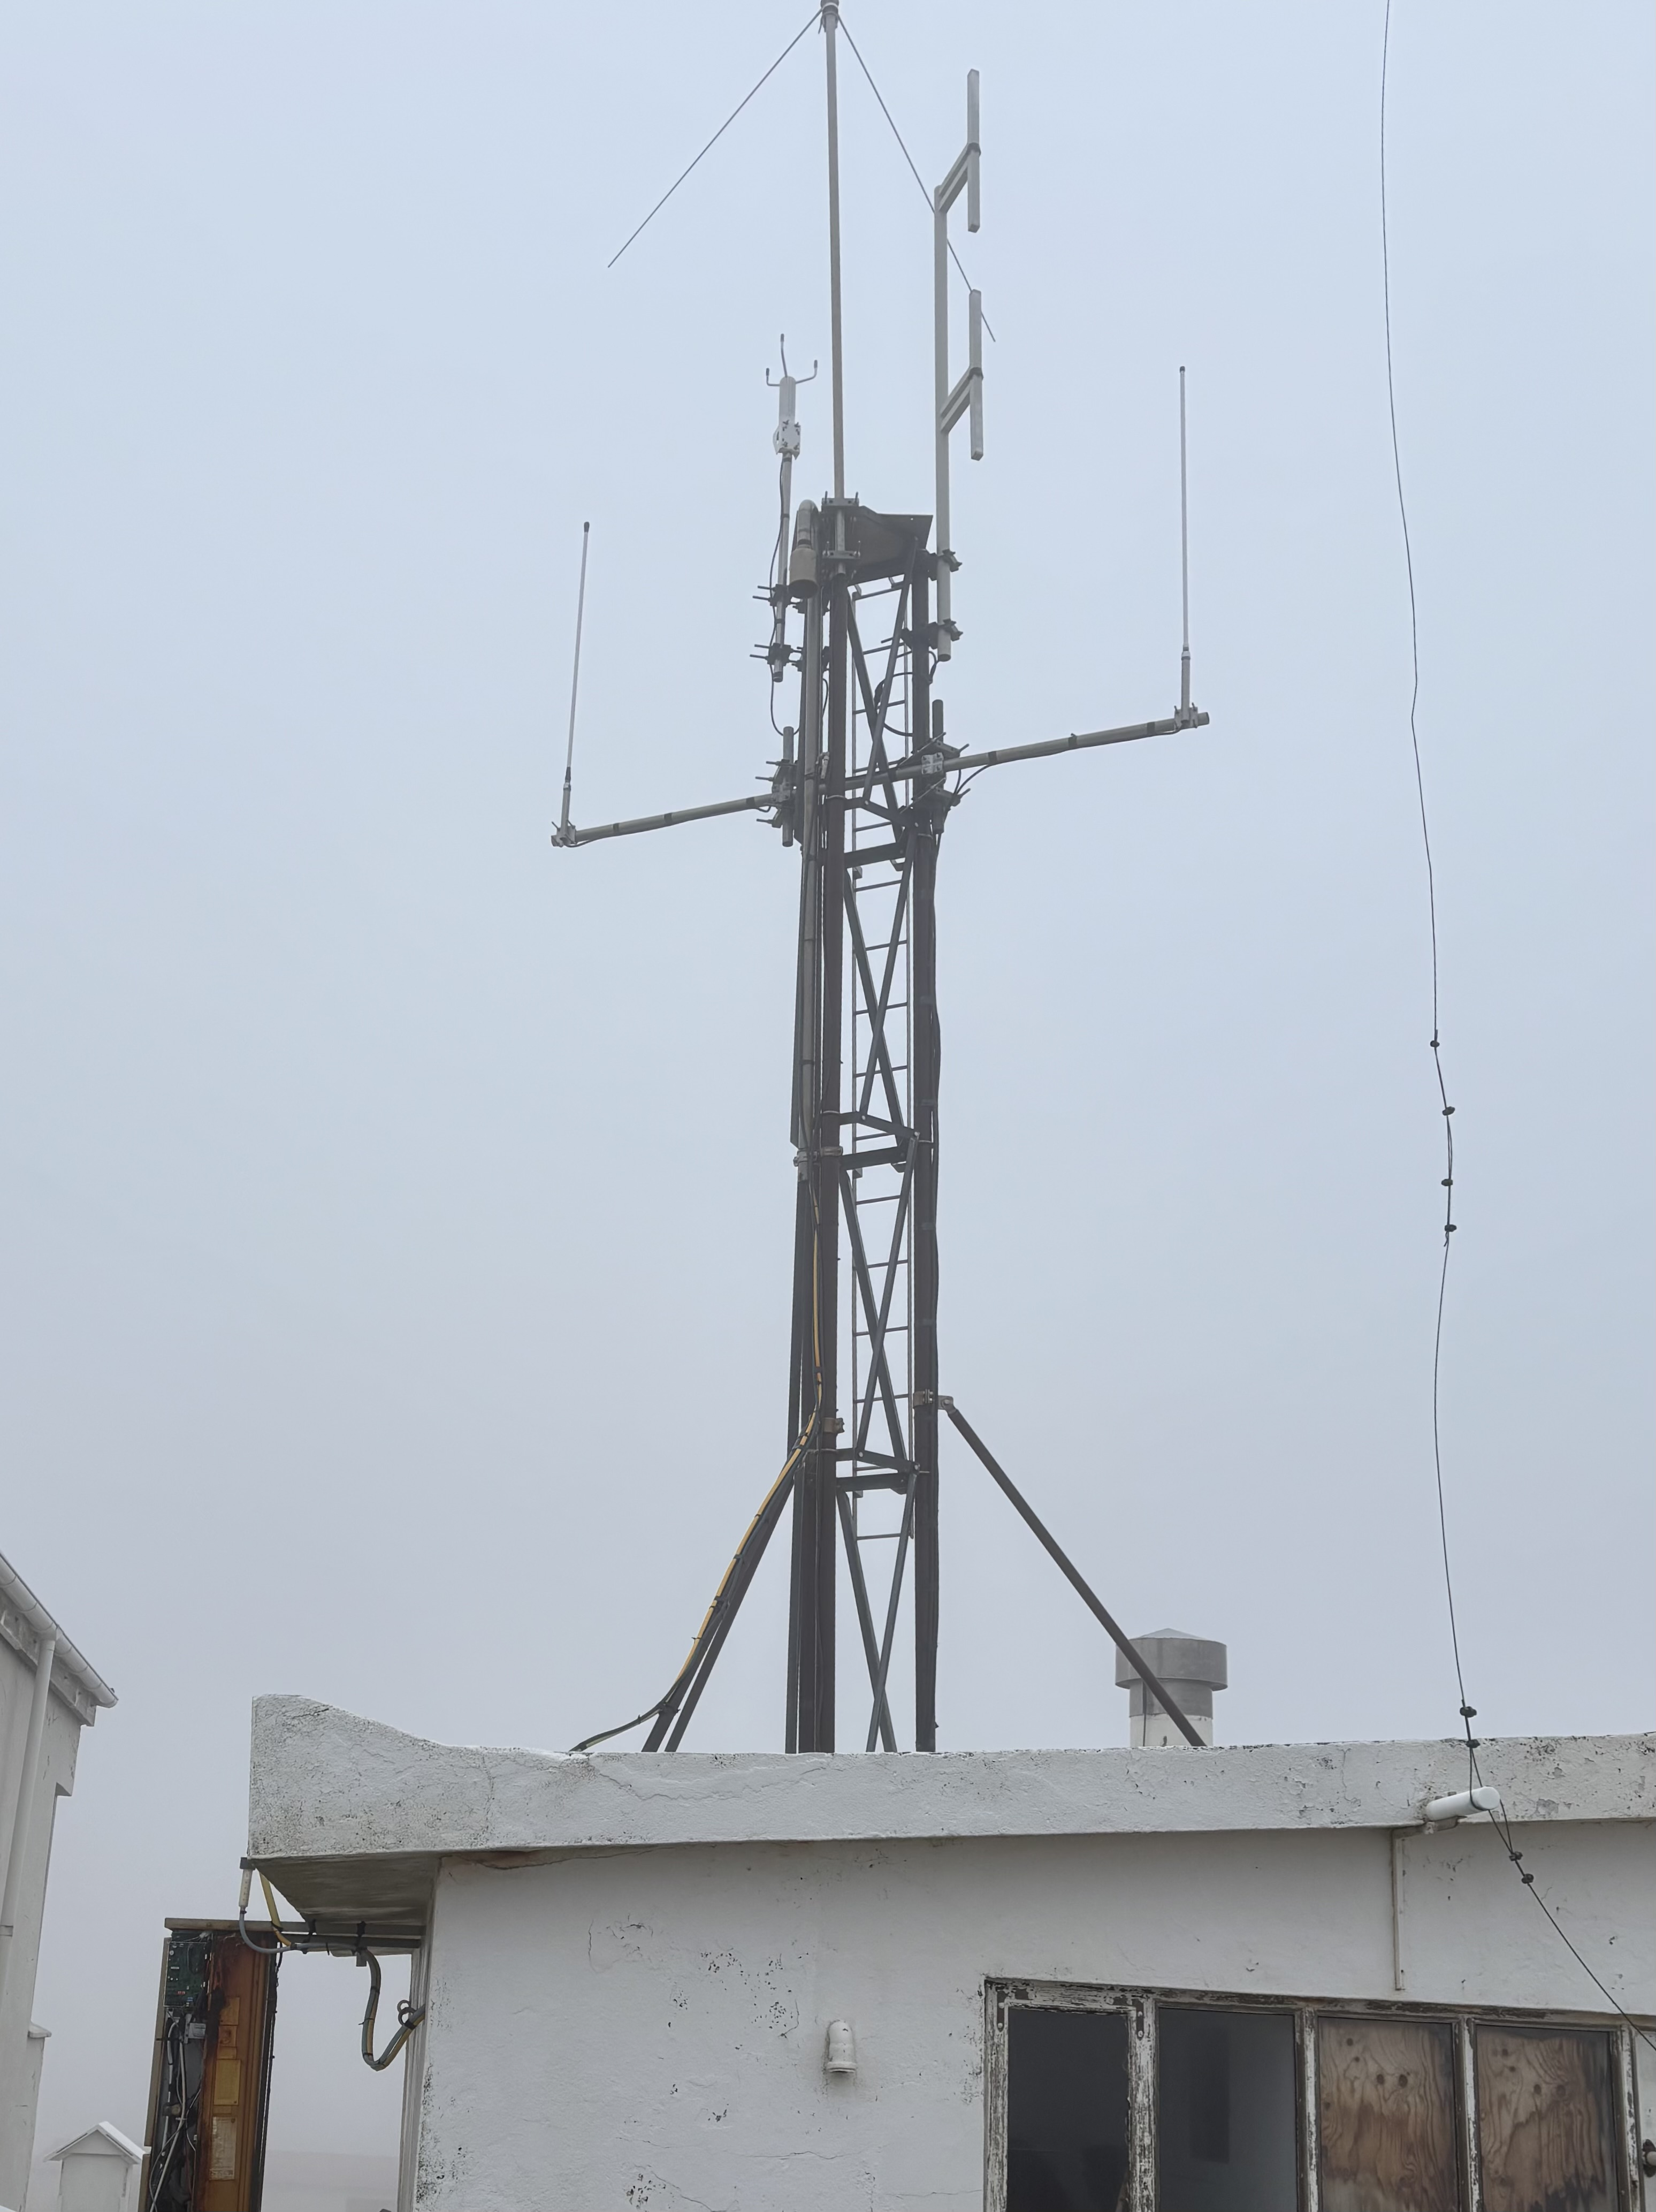
\includegraphics[scale=0.3]{Figures/storhofdi.jpeg}
  \caption[AWS at Stórhöfði in Vestmannaeyjar, south of Iceland.]{AWS at Stórhöfði in Vestmannaeyjar, south of Iceland. The anemometer can be seen as three pins in the upper-central area of the figure just slightly to the left.}
  \label{fig:storhofdi}
\end{figure}

\section{Automatic Weather Station Data}
Automatic weather stations (AWS) have been set up all around the world, including Iceland. AWSs might include a variety of sensors, such as barometers, thermometers, and anemometer along with solar panels (or other power source) and some kind of data logger. IMO provided measurements from AWSs across Iceland. One of the stations used in this study can be seen in Figure \ref{fig:storhofdi}. Not every station had consistently available data. Data from \nStationsMin AWSs were included looking at a period from \startDateVedur and ended in 2023. Of these \nStationsMin stations provided by IMO, \nVedurMin were IMO stations, with the anemometer at 10~m above ground, while the remaining \nVGMin stations were from \href{https://www.vegagerdin.is/}{the Icelandic Road and Coastal Administration (IRCA)}, with the anemometer at 6–7~m above ground \cite{vegagerdin_postur}. The locations of these weather stations are shown in Figure \ref{fig:aws_map}.

Data from these AWSs were stored in hourly files, which aggregate the original 10-minute files; measurement errors—unrealistic spikes known as “nails”—have been removed in most cases. Each record contains the following information: date and time; station number (convertible to coordinates using another dataset of Icelandic meteorological stations); average wind speed ($f$); wind gust ($f_g$); standard deviation of the wind gust; wind direction ($d$); and standard deviation of the wind direction.

These measurements began at the end of the 20th century with the installation of the first AWSs, and more stations have been added in subsequent decades.

\begin{figure}
    \centering
    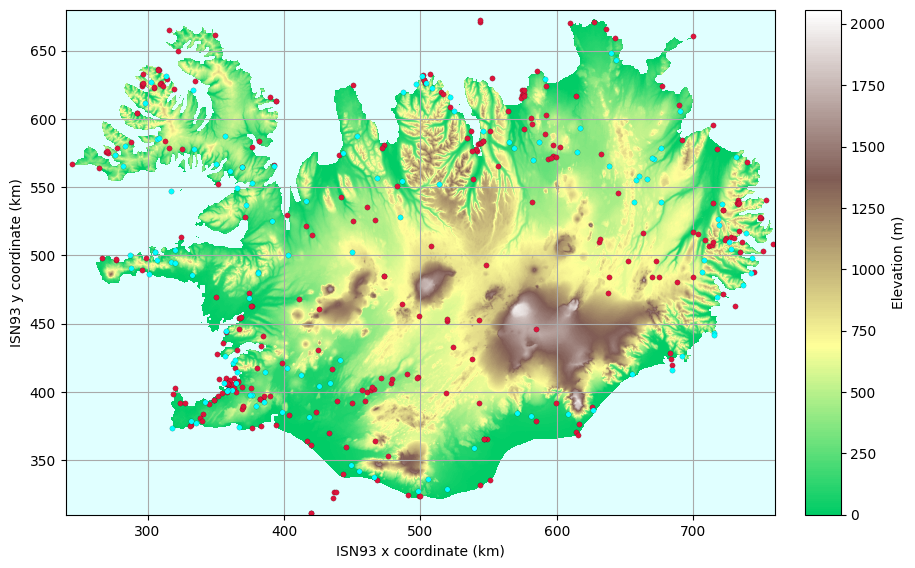
\includegraphics[scale = 0.6]{Figures/station_elevations.png}
    \caption[Locations of automatic weather stations in Iceland]{Locations of all 412 stations that were looked at in this study. Most of these were from IMO but over a hundred were from IRCA. IMO anemometers are placed at 10 meters above ground, while IRCA ones are placed at 6--7 meters above ground.}
    \label{fig:aws_map}
\end{figure}

\section{CARRA Data}
CARRA is a high-resolution atmospheric reanalysis produced by the Copernicus Climate Change Service and run by ECMWF. It covers two regions, a west region covering Greenland and Iceland and an east region covering the European Arctic. It has a 2.5 km horizontal resolution and dates from 1991 to the present, with monthly updates. CARRA provides three-hourly analysis fields and short-term forecasts (hourly for lead times under 6 h and three-hourly beyond) of surface and near-surface variables—wind, temperature, pressure, precipitation, etc. It is based on the HARMONIE-AROME limited-area NWP model, forced at its boundaries by ERA5 (ECMWF Re-Analysis v. 5) and enhanced by local observations to better represent complex terrain, land–sea contrasts, and sea-ice processes. It is updated monthly, with a latency of 2-3 months \cite{carra_information}.

The CARRA dataset covers all the IMO observations that fulfill criteria of consistent availability – the oldest observation is from \startDateVedur. The CARRA-West region covers a vastly larger area than the area of interest. This leads to having to store a large amount of data. To download CARRA data one has two options, a web interface or using an API client provided by CARRA. Using the API client is the only realistic option here, as there are thousands of requests made for different times. If using the API, it is possible to query a smaller area (such as a rectangular area around Iceland) given a set of coordinates, but this is not possible with the web interface.

The requests to the API were made at each available CARRA hour ([00, 03, 06, 09, 12, 15, 18, 21]) on a grid covering Iceland, for each available observation time. The downloaded data were interpolated to get values at the weather stations. CARRA contains several types of layers: single levels, model levels, height levels, and pressure levels. The data for this thesis was downloaded from height levels. They were requested at heights of 15, 250 and 500 meters above ground. For each point 4 parameters were requested, wind speed, wind direction, pressure, and temperature.

\section{Elevation data}
A GeoTIFF file containing a digital elevation model (DEM) for Iceland on a 20~m by 20~m grid was provided by the Icelandic Meteorological Office (IMO). The entire country is covered by this file, and its size is approximately 685\,MB.

The Python package \texttt{rasterio} is used, enabling rapid elevation lookup via its spatial indexing and affine‐transform capabilities. Elevation at specified geographic coordinates can be retrieved directly, and grid indices may be used for efficient access. Elevation for any exact location can be interpolated by fetching neighboring grid points.

\section{Combining data sources}

Three main data sources were used, each requiring querying, filtering, and merging to prepare the combined dataset. When handling hundreds of thousands of rows, code efficiency is essential: row-by-row iteration can increase execution time dramatically compared to vectorized operations.

The sources were provided in different formats: IMO measurement data in text files, elevation data in GeoTIFF, and CARRA reanalysis data in GRIB. To train the models, these datasets were combined into a single file using the IMO measurements as a reference. CARRA data are supplied on a rectangular grid with approximately 2.5~km spacing, while IMO observations are tied to specific station locations. Elevation data are on a 20~m by 20~m grid covering Iceland. Linear interpolation was applied to merge the sources.

\begin{figure}[h]
  \centering
  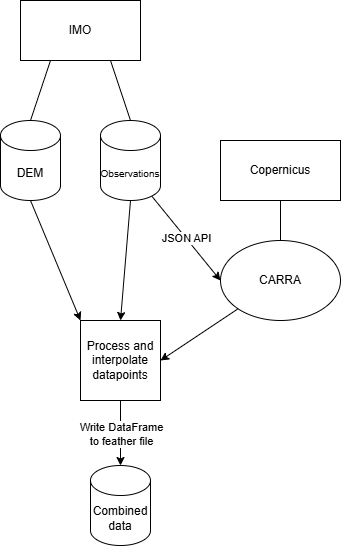
\includegraphics[scale=0.6]{Figures/data_combination.drawio.png}
  \caption{Flow chart illustrating the data-combination workflow}
  \label{fig:data_preprocessing_flow_chart}
\end{figure}

The merging procedure, shown in Figure \ref{fig:data_preprocessing_flow_chart}, was as follows: for each AWS observation, a query was constructed for the CARRA API by specifying year, month, day, hour, and spatial extent. Because the API returns all specified days when queried by hour, and all specified months when queried by day, monthly queries were issued for only the required days, retrieving all eight three-hourly time points (00, 03, 06, 09, 12, 15, 18, and 21~UTC). After downloading the requested variables at the desired pressure levels, point values were interpolated and appended to a pandas dataframe. The monthly GRIB files were then discarded before proceeding to the next month. This strategy reduced storage needs from several terabytes to under one gigabyte.

Elevation values from the GeoTIFF were interpolated in the same manner: the four surrounding grid points were used in a linear interpolation to estimate the elevation at each station location. These interpolated values were included in the dataframe, since topography influences both average wind speed and gustiness \cite{GNP_vidtal}.

\section{Comparison of observed and reanalysis wind speed}

Differences between reanalysis and measured wind speeds can be substantial. Absolute error increases with wind speed, while percentage error decreases. An overview of these errors by wind-speed range is shown in Table \ref{table:measuredVSReanalysis_wind_speed}.

\begin{table}[h]
  \centering
  \caption[Measured vs.\ reanalysis wind-speed errors]{Comparison of measured and reanalysis wind speeds using mean absolute error (MAE) and mean absolute percentage error (MAPE). Values for observed wind speeds below 1~m/s are excluded to avoid inflated MAPE values. Measured speeds are at 10~m above ground (IMO) or 6–7~m (IRCA); reanalysis speeds are at 15~m.}
  \label{table:measuredVSReanalysis_wind_speed}
  \begin{tabular}{cccc}
    \toprule
    $f$ & $n$ & MAE & MAPE \\
    \midrule
    $[1; 5[$     & 5,260,814  & 2.0 & 83.9\% \\
    $[5; 10[$    & 4,150,923  & 2.2 & 31.3\% \\
    $[10; 15[$   & 1,480,487  & 2.5 & 21.0\% \\
    $[15; 20[$   &   388,905  & 3.0 & 17.8\% \\
    $[20; 25[$   &    84,099  & 4.0 & 18.4\% \\
    $[25; \infty[$ &   20,288 & 6.6 & 23.0\% \\
    $[1; \infty[$  &11,385,516 & 2.2 & 53.7\% \\
    \bottomrule
  \end{tabular}
\end{table}

Next, the distribution of MAE by station is examined, considering station location and number of observations. Figure \ref{fig:station_mae_distribution} shows this distribution, and Table \ref{table:station_mae_distribution} lists the five stations with the lowest MAE and the five with the highest MAE.

\begin{figure}[h]
  \centering
  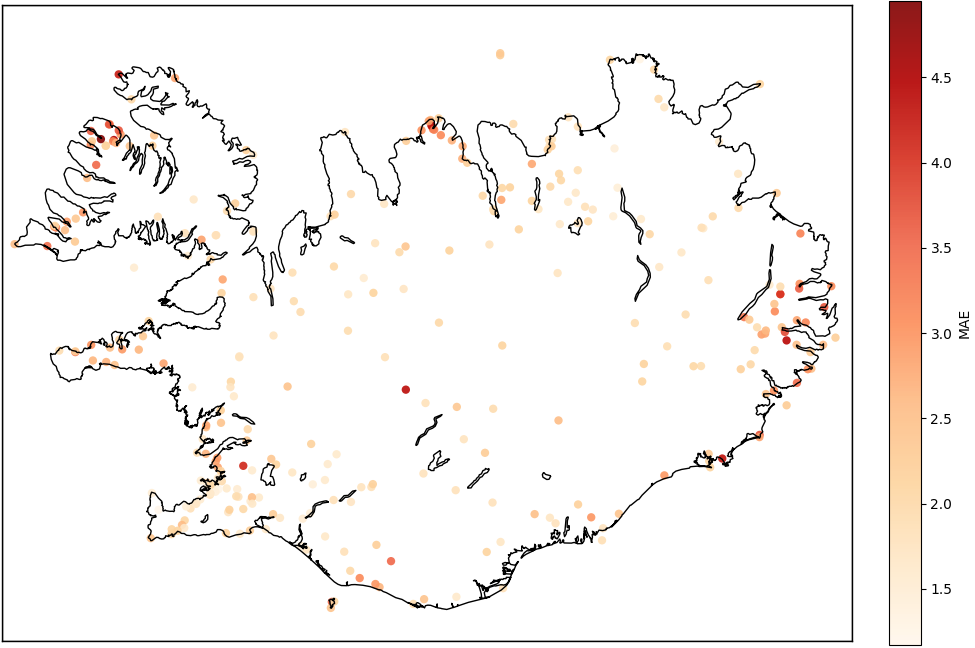
\includegraphics[scale=0.6]{Figures/MAEoverIceland.png}
  \caption[MAE distribution by station]{Distribution of mean absolute error (MAE) by station for all observed wind speeds.}
  \label{fig:station_mae_distribution}
\end{figure}

\begin{table}[h]
  \centering
  \caption[Station MAE extremes]{Mean absolute error (MAE) between reanalysis and observed wind speeds at the five stations with lowest and highest errors. The observation counts have been rounded.}
  \label{table:station_mae_distribution}
  \begin{tabular}{lcc}
    \toprule
    Station               & $n$     & MAE  \\
    \midrule
    Reykjavík Háahlíð     & 6,800   & 1.17 \\
    Keflavíkurflugvöllur  & 52,000  & 1.18 \\
    Reykjavík Víðidalur   & 14,000  & 1.23 \\
    Rif á Melrakkasléttu  & 13,000  & 1.29 \\
    Reykjavíkurflugvöllur & 56,000  & 1.29 \\
    \midrule
    Almannaskarð          &  4,000  & 4.30 \\
    Kerlingarfjöll        & 15,000  & 4.36 \\
    Fáskrúðsfjarðargöng   &  7,900  & 4.40 \\
    Seljalandsdalur       &  1,600  & 4.51 \\
    Botn í Súgandafirði   & 32,000  & 4.95 \\
    \bottomrule
  \end{tabular}
\end{table}

\section{Layout of combined data}\label{sec:layout}

Once data from all three sources have been retrieved and processed—including interpolation—they must be combined and formatted for modeling (training, validation, and testing). The starting point is a DataFrame containing AWS observations: average wind speed, wind gust, wind direction, station number, and coordinates. CARRA data are provided at selected height levels, each as a separate row in the CARRA DataFrame. Thus a single observation will span multiple rows, one per level. These rows are merged by time and station location, enabling AWS and CARRA data to be joined on station and time fields.

The DEM elevation data are handled by defining an upwind sector: a range of angles relative to the wind direction $d$ and radial distances from each station. Points within this sector are generated as shown in Code Listing \ref{code:sectorElevation}.

\begin{lstlisting}[
    style=Python,
    basicstyle=\small\ttfamily,
    caption={Generation of elevation points in the upwind sector},
    label=code:sectorElevation
]
angles = [(angle + (90 - d)) * pi/180 for angle in angleRange]
length_rng = [(exp(i * log(n + 1)/ k) - 1) * 1000 
              for i in range(1, k + 1)]
points = np.array([[(X + l * cos(angle), Y + l * sin(angle))
                    for angle in angles] for l in length_rng])   
\end{lstlisting}

The resulting DataFrame includes AWS measurements (our target), CARRA weather variables, and elevation points. An example of the combined data structure is shown in Table \ref{table:trainDataExample}.

\begin{table}[h]
    \centering
    \caption[Example of combined data structure]{Example of the combined data structure of features used for modeling. Data include derived variables Richardson number (Ri) and squared Brunt–Väisälä frequency ($N^2$), station altitude (meters above sea level), transformed wind direction (twd), wind speed (ws$_{15}$), wind direction (wd$_{15}$), temperature ($t_{15}$), pressure ($p_{15}$) (CARRA values at 15 m height), and elevation points (from DEM) in a sector pointing upwind.}
    \label{table:trainDataExample}
    \resizebox{\textwidth}{!}{
    \begin{tabular}{ccccccccccc}
        \toprule
        Ri & $N^2$ & \shortstack{station\\altitude} & twd & ws$_{15}$ & wd$_{15}$
        & $t_{15}$ & $p_{15}$ & $\text{elevation}_0$ & elevation$_1$ & \dots\\
        \midrule 
        -1.18 &  26700 & 100 & 1.5 & 10 & 5 & 0 & 100 & 2 & 4 & \dots\\
        \dots\\
        \bottomrule
    \end{tabular}
    }
\end{table}

The transformed wind direction is a proxy showing whether the wind is coming from land or sea. It is computed as the angle between the wind direction and a vector from the center of Iceland to the station.

The Richardson number and the Brunt–Väisälä frequency describe atmospheric stability, see Equations (\ref{eqn:Ri}) and (\ref{eqn:N}) \cite{richardson_number_skybrary,brunt_vaisala_freq_eumtrain,mean_gust_HA_HO}. These values are calculated using reanalysis data at two different height levels. Thus Ri refers to the Richardson number calculated between height levels 15m and 500m. Exactly the same notation is used with the Brunt–Väisälä frequency, except the square is used.
%
\begin{equation}
  \label{eqn:Ri}
  Ri = \frac{g \cdot d\theta \cdot dz}{\theta_{\textrm ave} \cdot dU^2} \unit{[]}
\end{equation}
%
\begin{equation}
  \label{eqn:N}
  N = \sqrt{\frac{g \cdot d\theta }{\theta_{\textrm ave} \cdot dz}} \unit{[Hz]}
\end{equation}
%
Here, $g$ is gravitational acceleration; $d\theta$ the potential temperature difference between levels; $dz$ the height difference; $\theta_{\mathrm{ave}}$ the average potential temperature; and $dU$ the wind-speed difference. Lower Ri indicates greater turbulence, with typical values between 0.1 and 10, and values below 1 signifying significant turbulence \cite{richardson_number_skybrary}. Negative $N^2$ denotes instability, as an air parcel will accelerate away from its original position \cite{brunt_vaisala_freq_eumtrain}. The potential temperature is computed as:
%
\begin{equation}
  \label{eqn:potential_temp}
  \theta = T\left(\dfrac{P0}{P}\right)^{R/c_p}
\end{equation}
%
where $P$ is the pressure and $R = 287$ and $c_p = 1004$ are the specifc gas constant and the specific heat capacity of air.

Since Ri and $N^2$ are derived from reanalysis variables, they add limited new information compared to the raw data, but they can reduce input dimensionality and improve model explainability via Shapley-value analysis \cite{shapley_information}. Shapley values assess feature importance by evaluating all possible feature subsets—an operation of computational complexity $2^n$. In practice, approximations are used but can still be costly for large models. Because $dU$ appears squared in the denominator of Ri, if the wind-speed difference between levels is very small, Ri can become arbitrarily large, potentially distorting predictions.

\section{Distributions of observed and reanalysis data}

CARRA reanalysis data may exhibit bias or systematic differences when compared to measurements. Figure \ref{fig:obs_carra_wind_speeds} shows the distributions of observed and reanalysis wind speeds. Although the shapes are similar, reanalysis values tend to be higher.

\begin{figure}[ht]
  \centering
  \begin{subfigure}[b]{0.8\textwidth}
    \centering
    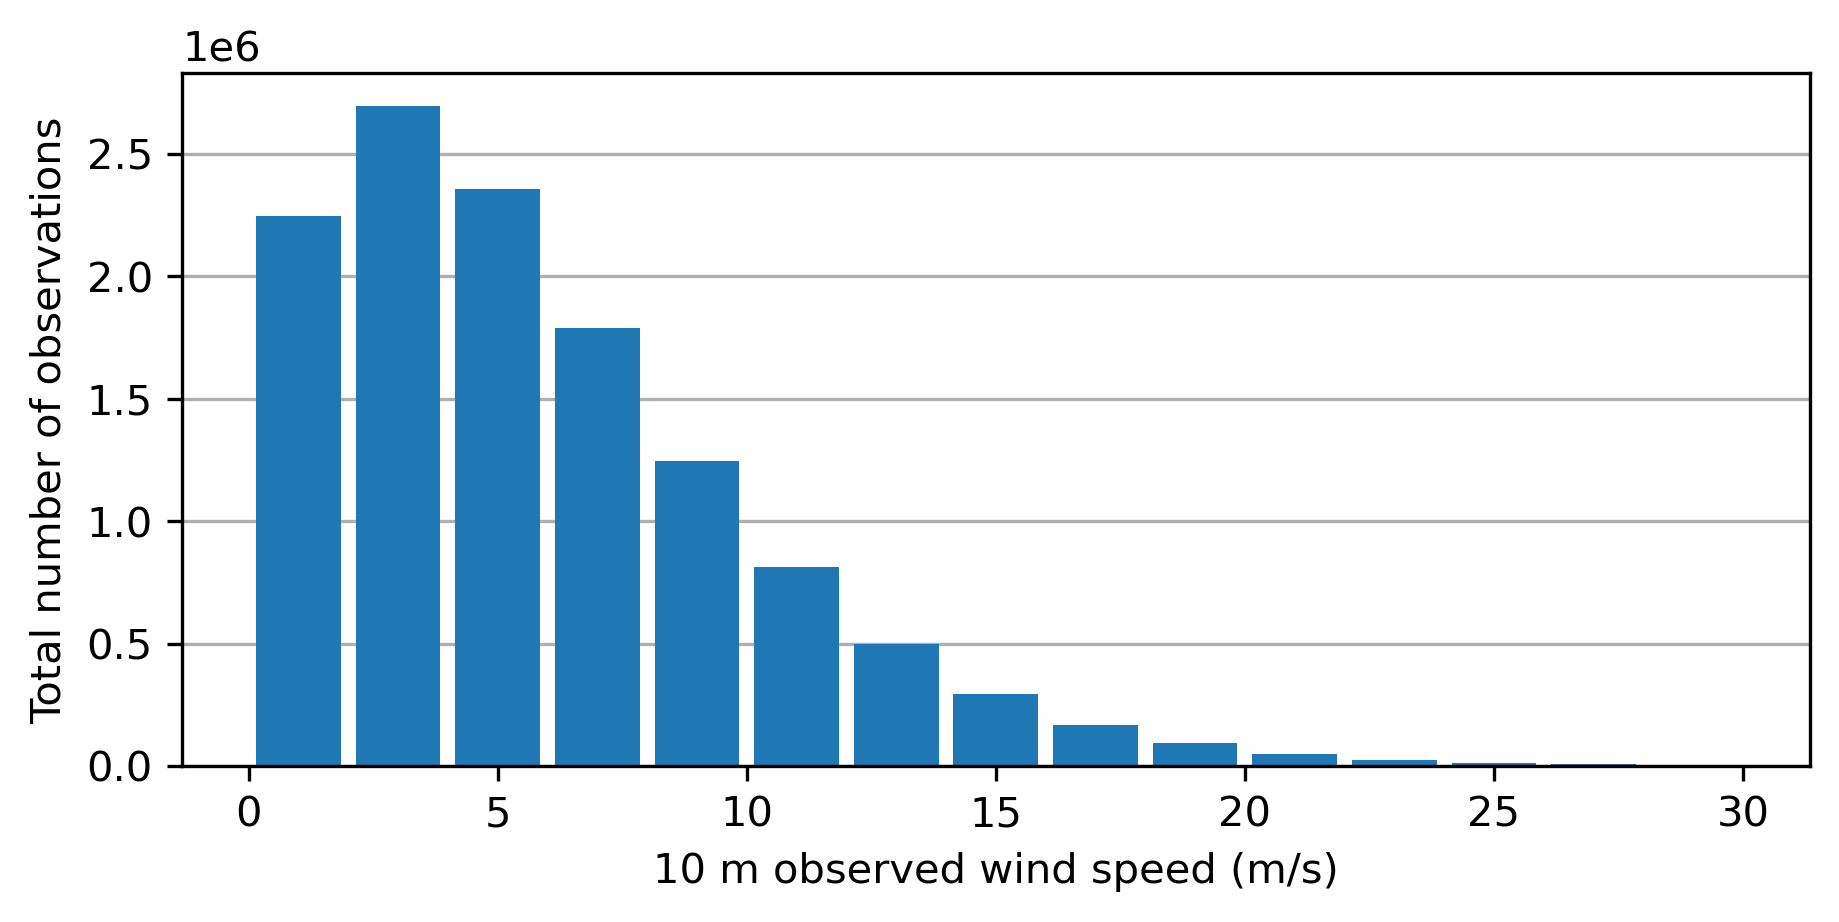
\includegraphics[width=\textwidth]{Figures/obs_wind_speeds.png}
    \caption{Histogram of observed wind speeds from IMO and IRCA at all stations, sampled at 3-hour intervals (00,~03,~06,~…~,21~UTC).}
    \label{fig:obs_wind_speeds}
  \end{subfigure}
  
  \vspace{0.5cm}
  
  \begin{subfigure}[b]{0.8\textwidth}
    \centering
    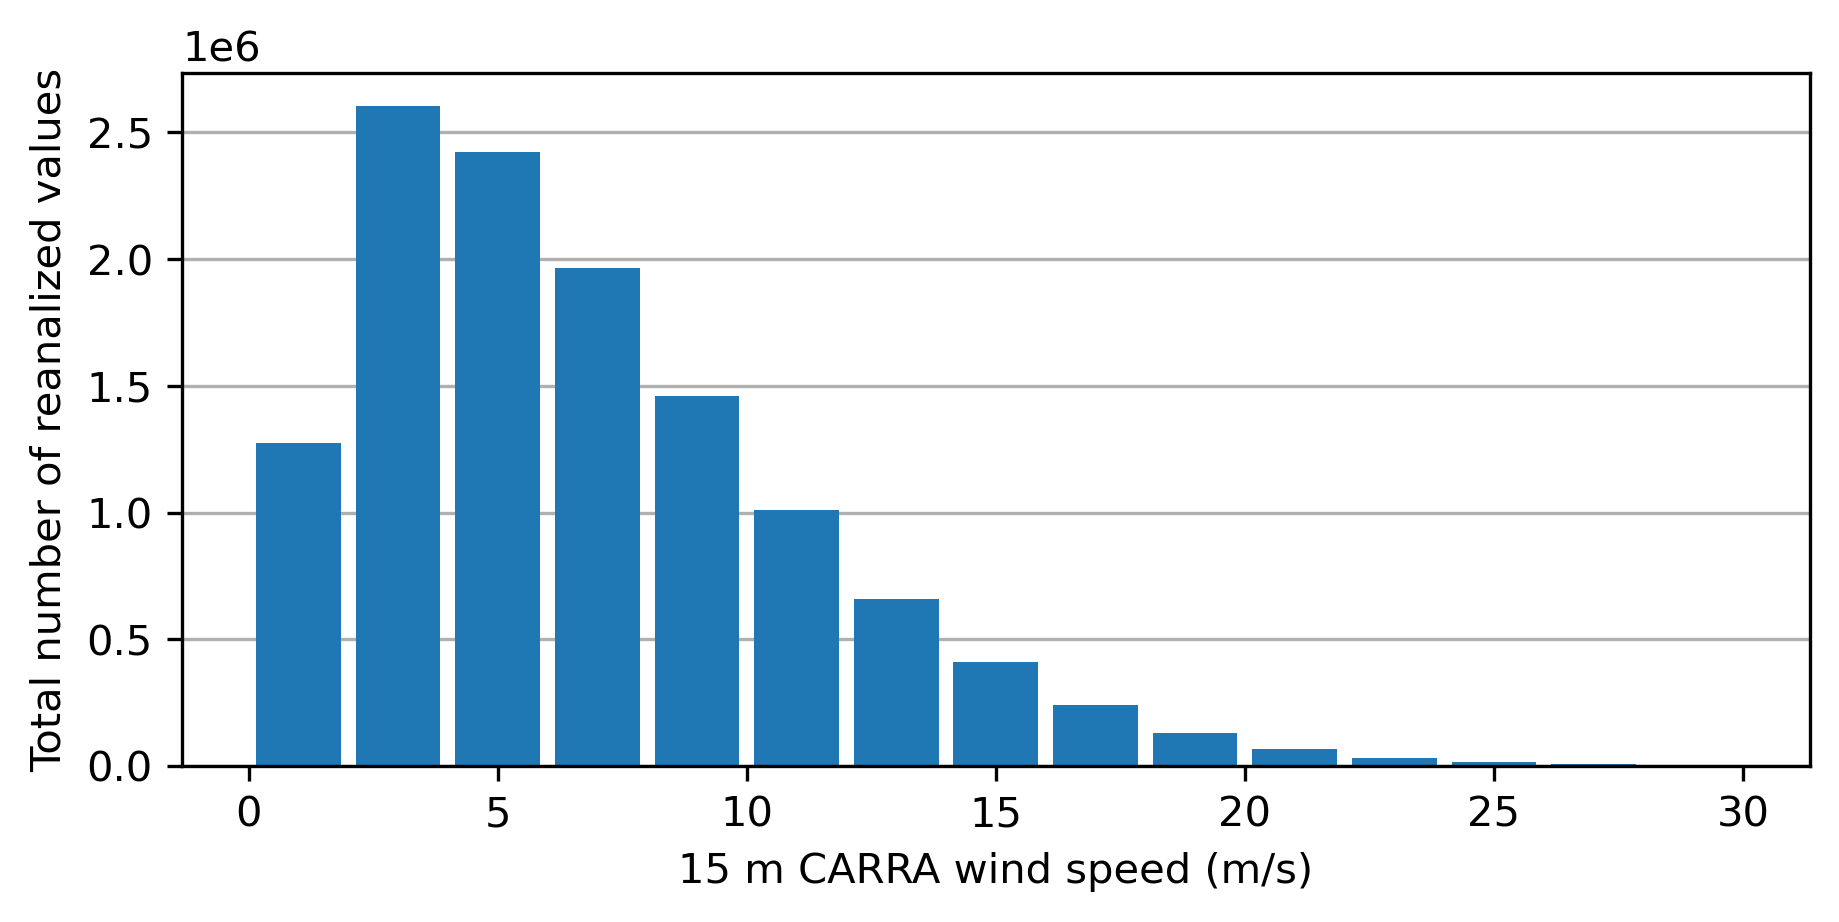
\includegraphics[width=\textwidth]{Figures/carra_wind_speeds.png}
    \caption{Histogram of interpolated CARRA wind speeds at station locations on a 2.5~km grid and 3-hour intervals.}
    \label{fig:carra_wind_speeds}
  \end{subfigure}
  
  \caption{Comparison of observed and reanalysis wind-speed distributions. CARRA values are spatially interpolated by linear weighting of surrounding grid points.}
  \label{fig:obs_carra_wind_speeds}
\end{figure}

\begin{figure}[ht]
  \centering
  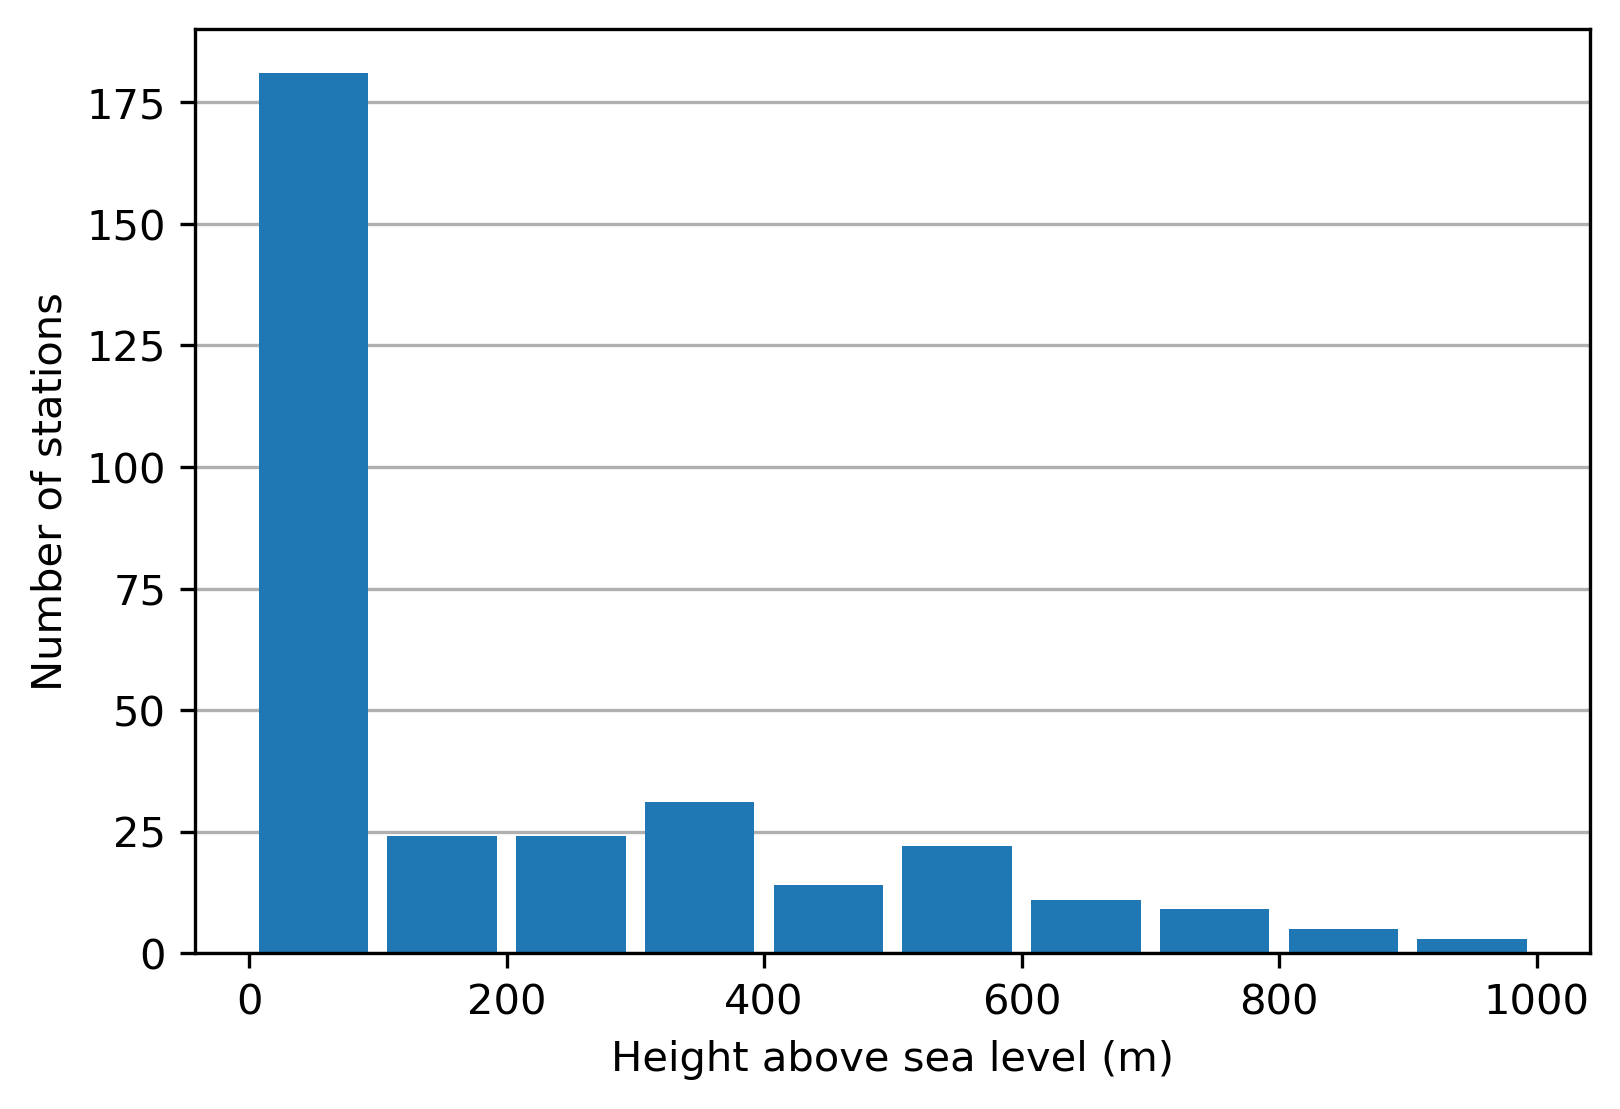
\includegraphics[width=0.8\textwidth]{Figures/station_heights.png}
  \caption{Distribution of weather station altitudes above sea level. One outlier near 2000~m was excluded due to limited and inconsistent data.}
  \label{fig:station_heights}
\end{figure}

\begin{figure}[ht]
  \centering
  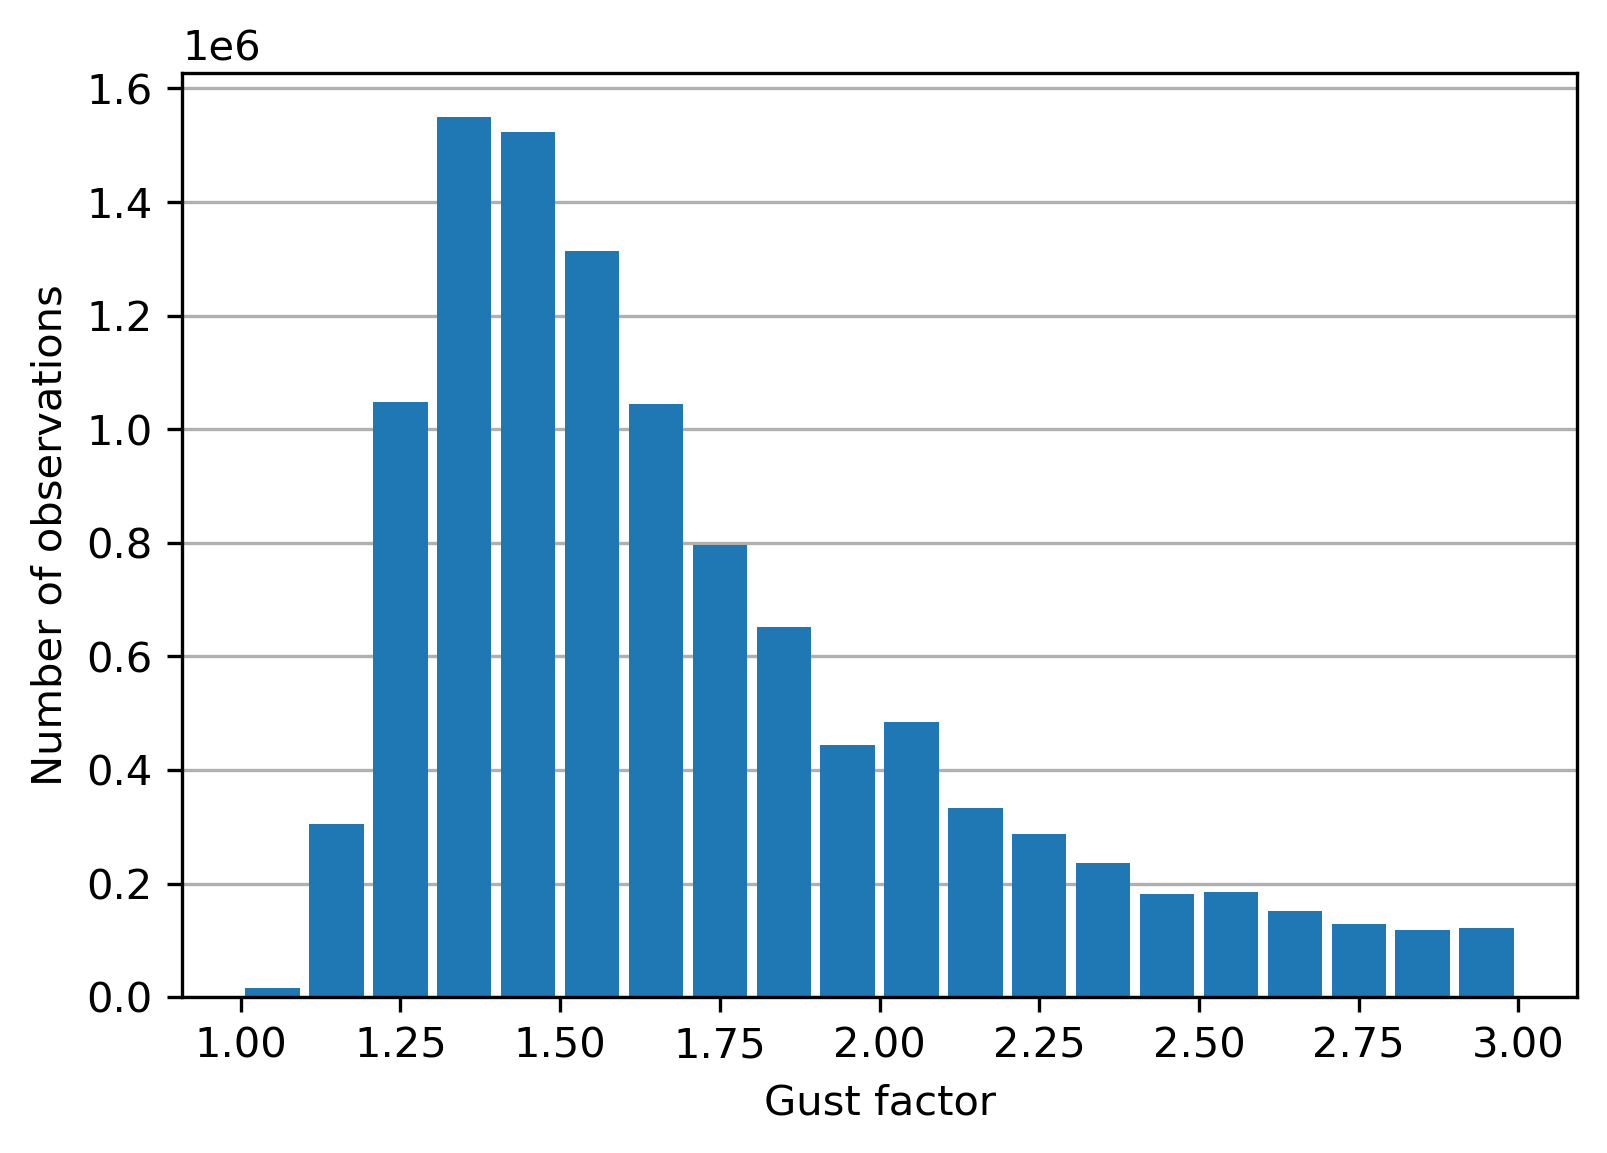
\includegraphics[width=0.8\textwidth]{Figures/gust_factor_2025.png}
  \caption{Histogram of gust factors. By definition, gust factor $\ge1$; most values lie between 1.2 and 2. The gust factor declines as wind speed increases.}
  \label{fig:gust_factors}
\end{figure}

\section{Model architecture}
\label{sec:model_architecture}

The network consists of $n$ fully connected layers, with $n$ around 10. Each hidden layer has the same number of units and is followed by batch normalization. A dropout layer with rate 50\% is applied after the final hidden layer. A dense output layer with one unit produces the predicted gust factor. A grid search was used to find the hyperparameters that minimize the loss. Hyperparameters are settings defined before training begins \cite{hyperparameters_definition}. They include the number of units per layer, the number of layers, the number of training epochs, batch size, optimizer choice, and regularization penalty. The ranges tested are listed in Table \ref{table:gridSearchHyperparameters}.


\begin{table}[h]
    \centering
    \caption[Hyperparameter search with Hyperband]{Hyperparameter search was performed using the Hyperband algorithm, which begins by sampling configurations at random and then focuses on the most promising ones. The table shows the ranges tested and the best-performing combination. Unlike random search, Hyperband does not impose a fixed limit on the number of trials.}
    \label{table:gridSearchHyperparameters}
    \begin{tabular}{lll}
        \toprule
        Parameter & Range of values & Selected\\
        \midrule
        Layers &  min\_value = 4, max\_value = 15, step = 1 & \textbf{10}\\
        Units &  min\_value = 32, max\_value = 512, step = 32 & \textbf{64}\\
        Penalties & min\_value = 1e-5, max\_value = 1, sampling = log & \textbf{1e-4}\\
        Epochs & min\_value = 10, max\_value = 1000, step = 10 & \textbf{250}\\
        Optimizers & Adam, RMSprop, Adamax & \textbf{Adamax}\\
        Activation & ReLU, ELU, tanh & \textbf{ReLU}\\
        \bottomrule
    \end{tabular}
\end{table}

As mentioned, Hyperband doesn't set a hard upper limit to the number of epochs it will train in total. When using the \href{https://keras.io/api/keras_tuner/tuners/hyperband/}{Hyperband class} several factors can be set. One of interest here is the Hyperband iterations argument. This determines how often the Hyperband algorithm is run and defaults to 1. For each iteration the epochs are distributed between tries (that is each set of hyperparameters) with the total amount of epochs approximately $n_{epochs} = max_{epochs} * log^2(max_{epochs})\approx 10^4$, where $max_{epochs} = 1000$ gives the maximum number of epochs that one set of hyperparameters can be trained for. Searching a space generally takes a lot of time but this drastically improves on grid search. If each epoch takes around 10 seconds to run then the total search would take around 28 hours on a shared resource. This is resource-intensive and cannot be repeated often. Another question that remains is whether the ranges given are optimal.

As noted, Hyperband does not impose a fixed limit on the total number of training epochs. When using the \href{https://keras.io/api/keras_tuner/tuners/hyperband/}{Hyperband tuner}, the Hyperband iterations parameter controls how many times Hyperband is run and defaults to 1. On each run, the total number of epochs is distributed across the hyperparameter trials. The total number of epochs is approximately
%
\begin{equation*}
n_{\mathrm{epochs}} = \text{max\_epochs} \times \bigl(\log(\text{max\_epochs})\bigr)^2 \approx 10^4
\end{equation*}
%
for $ \text{max\_epochs} = 1000$. Although this method is more efficient than grid search, if each epoch takes about 10 seconds, a complete Hyperband search can still require about 28 hours on shared resources, making repeated searches impractical. It remains unclear whether the current hyperparameter ranges are optimal.
% Chapter Template

\chapter{Model Architecture and Training}

\label{Chapter3}

\section{Model structure}
The structure of the neural network is such that it contains some number $n$ of fully connected layers and batch normalization for each layer, along with regularization. All of these layers have the same number of units. The last layer has a dropout of 50\%. In addition to these layers there is one more output layer. This is simply a dense layer with 1 unit. A grid search was performed to determine the hyperparameters that minimize the loss. Hyperparameters are parameters that are set before the training begins\cite{hyperparameters_definition}. These hyperparameters include number of units in each layer, number of epochs to train for, number of layers, batch size, optimizer and penalty to enforce in the regularization. The possible combinations tried can be seen in Table \ref{table:gridSearchHyperparamters}.

\begin{table}[h]
    \centering
    \caption[Hyperparameter search with best performing combination.]{Hyperparamter search with best performing combination shown. Hyperparameter search was done using hyperband algorithm that initially searches randomly for the best parameters but then hones in on what is working and as such is neither exhaustive nor completely random. This means that a hard upper limit will not be set on the number of combinations to try like with randomsearch.}
    \label{table:gridSearchHyperparamters}
    \begin{tabular}{ccc}
        \toprule
        Parameter & Range of values & Selected\\
        \midrule
        Layers &  min\_value = 4, max\_value = 15, step = 1 & \textbf{10}\\
        Units &  min\_value = 32, max\_value = 512, step = 32 & \textbf{64}\\
        Penalties & min\_value = 1e-5, max\_value = 1, sampling = log & \textbf{1e-4}\\
        Epochs & min\_value = 10, max\_value = 1000, step = 10 & \textbf{250}\\
        Optimizers & Adam, RMSprop, Adamax & \textbf{Adamax}\\
        Activation & ReLU, ELu, tanh & \textbf{ReLU}\\
        \bottomrule
    \end{tabular}
\end{table}

As mentioned, hyperband doesn't set a hard upper limit to the number of epochs it will train in total. When using the \href{https://keras.io/api/keras_tuner/tuners/hyperband/}{hyperband class} several factors can be set. One of interest here is the $hyperband_iterations$ argument. This determines how often the hyperband algorithm is run and defaults to 1. For each iteration the epochs are distributed between tries (that is each set of hyperparameters) with the total amount of epochs approximately $n_{epochs} = max_{epochs} * log^2(max_{epochs})\approx 10^4$, where $max_{epochs} = 1000$ gives the maximum number of epochs that one set of hyperparameters can be trained for. Searching a space generally takes a lot of time but this drastically improves on gridsearch. If each epoch takes around 10 seconds to run then the total search would take around 28 hours on a shared resource. This is resource intensive and cannot be repeated often. Another question that remains is whether the ranges given are optimal.

\section{Model Training}
To determine the required number of epochs a high number of epochs can be selected and the loss plotted. These plots can be seen in Figures (\ref{fig:loss_plot_wo_elevation}, \ref{fig:loss_plot_w_elevation}). Looking at these two plots, training loss decreases for over 1900 epochs in both plots, while the validation loss stops decreasing at around 200 epochs for DEM model and 1800 epochs for model without DEM. This is unexpected. The DEM model has vastly more parameters and as such should contain more useful information to be learned, which one might expect to take longer to learn. This does not seem to be the case. The DEM model only gets trivially better after 1000 epochs while the non DEM model keeps meaningfully improving until around 1800 epochs. With respect to time constraints of shared resources models were trained for 250 epochs.

\begin{figure}
    \centering
    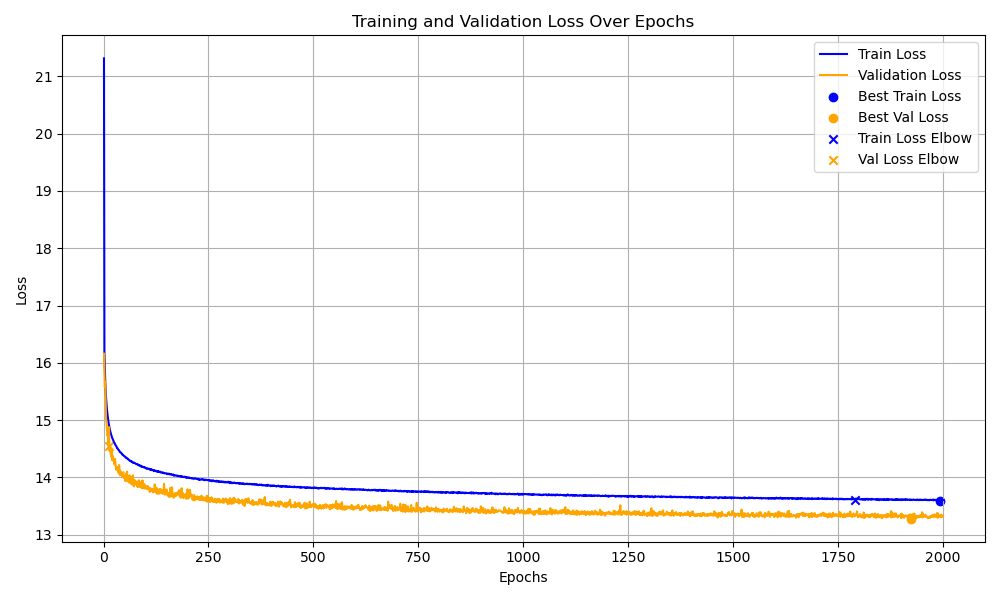
\includegraphics[scale = 0.6]{Figures/loss_plot_wo_elevation.png}
    \caption[Loss plot of model trained for 2000 without DEM.]{Loss plot of model trained for 2000 without DEM.}
    \label{fig:loss_plot_wo_elevation}
\end{figure}


\begin{figure}
    \centering
    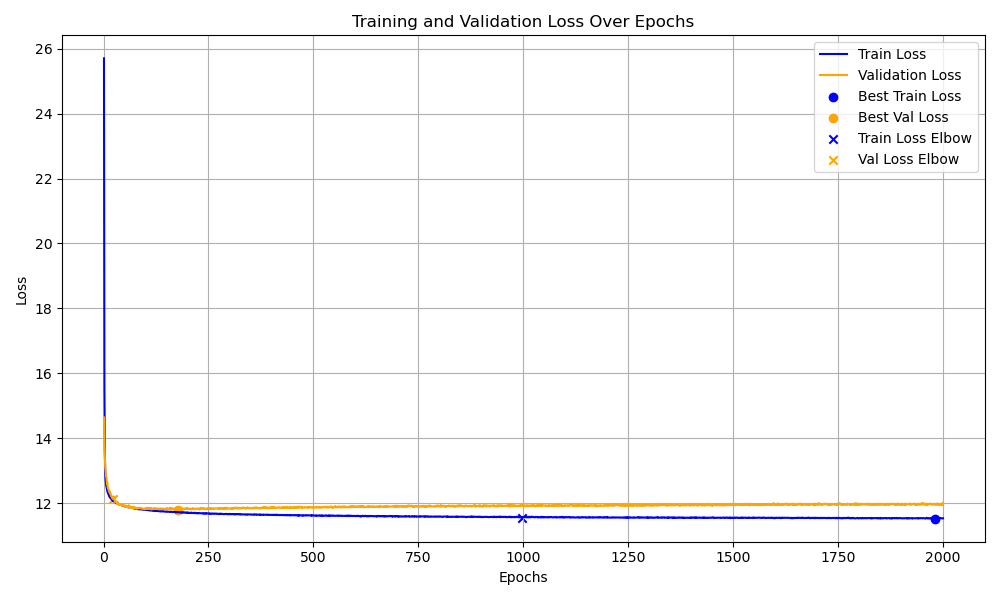
\includegraphics[scale = 0.6]{Figures/loss_plot_w_elevation.png}
    \caption[Loss plot of model trained for 2000 with DEM.]{Loss plot of model trained for 2000 with DEM.}
    \label{fig:loss_plot_w_elevation}
\end{figure}
% Chapter Template

\chapter{Model architecture} % Main chapter title

\label{Chapter4} % Change X to a consecutive number; for referencing this chapter elsewhere, use \ref{ChapterX}

%----------------------------------------------------------------------------------------
%	SECTION 1
%----------------------------------------------------------------------------------------

\section{Model structure}
The structure of the neural network is such that it contains some number $n$ of fully connected layers and batch normalization for each layer, along with regularization. All of these layers have the same number of units. The last layer has a dropout of 50\%. In addition to these layers there is one more output layer. This is simply a dense layer with 1 unit. A grid search was performed to determine the hyperparameters that minimize the loss. Hyperparameters are parameters that are set before the training begins\cite{hyperparameters_definition}. These hyperparameters include number of units in each layer, number of epochs to train for, number of layers, batch size, optimizer and penalty to enforce in the regularization. The possible combinations tried can be seen in Table \ref{table:gridSearchHyperparamters}.

\begin{table}[h]
    \centering
    \caption[Hyperparamter search with best performing combination.]{Hyperparamter search with best performing combination shown. Hyperparameter search was done using hyperband algorithm that initially searches randomly for the best parameters but then hones in on the what is working and as such is neither exhaustive nor completely random. This means that an upper limit will nont be set on the number of combinations to try like with randomsearch.}
    \label{table:gridSearchHyperparamters}
    \begin{tabular}{c|c|c}
        Parameter & Range of values & Selected\\\hline
        Layers &  min\_value = 4, max\_value = 15, step = 1 & \textbf{11}\\\hline
        Units &  min\_value = 32, max\_value = 512, step = 32 & \textbf{64}\\\hline
        Penalties & min\_value = 1e-4, max\_value = 1, sampling = log & \textbf{0.000168}\\\hline
        Epochs & min\_value = 50, max\_value = 1000, step = 50 & \textbf{750}\\\hline
        Optimizers & Adam, RMSprop, Adamax & \textbf{RMSProp}\\\hline
        Activation & ReLU, ELu, Softmax & \textbf{eLU}\\\hline
    \end{tabular}
\end{table}

\section{Feature selection and importance}
Using the three datasources, a model is trained. The data from IMO only represents the ground truth and is not used as part of the training data. The gust ($f_g$) and wind speed ($f$) are used to calculate the target gust factor. All weather parameters used in predictions come from the CARRA reanalysis data, with variables wind speed, wind direction, temperature, pressure. All of these variables are queried in three height levels (15, 250, 500 meters above ground) at the location of a given weather station. The second data source for the training data, is the elevation data. Using the GeoTIFF file that IMO provided, several different landscape elevation distributions were looked at. A sector upwind, a sector upwind and downwind as well as a circle surrounding a weather station.

To begin with all the available parameters were used to train the model along with the derived variables. This is done to be able to then use tools such as Shapley to see which features are impacting the predictions. Using Shapley values to see which features, will then enable the exclusion of features that don't affect the model prediction and simplify the training data. This means starting with much higher dimensionality of our training data and reduce it as much as possible without impacting our results. This crystallizes in the landscape points. Starting with $n$ points that describe the elevation of the landscape around our weather station. This $n$ might be in the hundreds. Looking at concentric circles outward from a given weather station, there might be 10 circles (largest with radius 20 km), each with 72 points (5° spacing) and end up with 720 points for the landscape. This might slow down training. In addition, certain landscape features might be more important than others. There might be a large mountain up- or downwind of a given weather station, that might be the most important feature. To address this principal component analysis (PCA) is used to try to reduce the dimensionality of our landscape elevation data. PCA is a statistical procedure that allows the summarization of multivariate data to lower dimension and thus can ease visualization or increase speed of training a complex model with only minimal adverse effect to performance\cite{pca_information}.

Using all the variables from CARRA, along with the two derived factors ($Ri$, $N$) and two sectors (upwind and downwind) downscaled to 10 features using PCA, the feature importance can be seen in Figure \ref{fig:ShapleyWaterfallFirstTry}. The waterfall graph in Figure \ref{fig:ShapleyWaterfallFirstTry} shows that the Richardson number for higher levels is most important.

\begin{figure}[h]
    \centering
    \includegraphics[scale = 0.6]{Figures/shap_bar_nn_256_example100.png}
    \caption[Feature importance of a neural network.]{Feature importance of a neural network as described with 5 hidden layers and 256 units in each}
    \label{fig:ShapleyWaterfallFirstTry}
\end{figure}
\chapter{Results}
\label{Chapter5}
\section{Results}
A baseline model was constructed. This model looked at the gust factor for some training data and took the average of this and predicted this average everytime. Several baseline guesses were created based on a lower limit assigned to the average wind speed limit (AWSL). As the average wind speed increases, then the variability in gust as a percentage decreases\cite{mean_gust_HA_HO}. This means looking at a subset of the data where the AWSL is higher, a better result can be expected. The results show this. Several different AWSL were used for the baseline model, as can be seen in table \ref{table:results}. This sets a goal. A model that does not significantly improve on this baseline suggests either failure to capture essential patterns in the data or that the data itself may lack the necessary information for substantial improvements upon the baseline. Using the previously described neural network architecture setups for each AWSL, with and without landscape elevation information, MAPE was determined. The results can be seen in Table \ref{table:results}.

\begin{table}[h]
    \caption[Model results for different AWSL]{MAPE for each average wind speed limit with and without landscape elevation in a 30° sector around the point of interest into the direction of the reanalysis wind. The influence of adding elevation data seems to reduce the error. The percentage error is higher for lower wind speeds and thus observing the error for different lower bound of wind speed will produce different results. This lower bound is determined using the reanalysis wind speed at 15 meters ($ws_{15}$).}
    \label{table:results}
    \centering
    \begin{tabular}{lccc}
        \toprule
        \textbf{AWSL} & \textbf{MAPE} & &\\ 
        $[m/s]$ & \textit{Baseline} &  \textit{Without DEM} & \textit{With DEM} \\
        \midrule
        $\geq 0$ & 39.2\% & 19.7\% & 18.6\% \\
        $\geq 5$ & 28.1\% & 15.9\% & 14.1\%\\
        $\geq 10$ & 23.9\% & 13.6\% & 11.5\%\\
        $\geq 15$ & 23.2\% & 13.0\% & 10.6\%\\
        $\geq 20$ & 24.7\% & 13.6\% & 11.1\%\\
        $\geq 25$ & 27.7\% & 15.7\% & 12.9\%\\
        \bottomrule
    \end{tabular}
\end{table}

%m/s & $ws_{15}$ & f & $ws_{15}$ & f & $ws_{15}$ & f\\
%$\geq 0$ & 39.2\% & 39.2\% & 19.7\% & 15.9\% & 18.6\% & 15.3\%\\
%$\geq 5$ & 28.1\% & 14.8\% & 15.9\% & 9.9\% & 14.1\% & 9.4\%\\
%$\geq 10$ & 23.9\% & 11.1\%& 13.6\% & 7.6\% & 11.5\% & 7.4\%\\
%$\geq 15$ & 23.2\% & 9.3\% & 13.0\% & 7.0\% & 10.6\% & 6.4\%\\
%$\geq 20$ & 24.7\% & 8.2\% & 13.6\% & 6.3\% & 11.1\% & 5.8\%\\
%$\geq 25$ & 27.7\% & 7.3\% & 15.7\% & 5.8\% & 12.9\% & 5.5\% \\
%7.5 & 25.3\% & 12.6\% & 14.5\% & 8.6\% & 12.5\% & 8.6\%\\
%12.5 & 23.3\% & 10.1\% & 13.1\% & 7.1\% & 11.0\% & 6.9\%\\
%17.5 & 23.7\% & 8.7\% & 12.8\% & 6.4\% & 10.5\% & 6.1\%\\
%22.5 & 26.1\% & 7.8\% & 14.5\% & 6.1\% & 12.6\% & 5.7\%\\

This is some improvement upon the baseline error, with a decrease in error from 23.9\% to 13.6\% and 10.6\% for the baseline, model without DEM and with model with DEM for 10 m/s cutoff. The power generated by wind mill increases with wind speed cubed\cite{wind_power}. The highest wind gusts in Iceland are around 70 m/s. Knowing the gust factor with half as much error as before can allow better anticipation and thus spare turbines for high wind gusts. Another way to look at the error improvement is by station. No location data was directly included in the training data. In Table \ref{table:station_mae_distribution} the mean absolute error of predicted average wind speed and measured average wind speed can be seen for the extreme values. A question to ask is it possible to achieve better results when only looking at a single station?

\begin{table}[h]
    \caption[Model result by station]{The MAPE results for selected stations of interest, both when training for the specific site and when the stations are a part of the general data. For every station the AWSL is set at 10 m/s. In training for a single station at a time, some site specific information can be gauged. This does not mean that the a better result can be reached for that site. Factors such as the number of datapoints at given location can significantly impact the result. This table uses the measured wind speed to determine the cut off for data points. This leads to some data leakage and an increased performance compared to using the reanalysis CARRA speed for cut off.}
    \label{table:specific_sites}
    \centering
    \begin{tabular}{lccc}
        \toprule
        \textbf{Station name} & \textbf{Number of measurement points} & \multicolumn{2}{c}{\textbf{MAPE}}\\
        & & General training & Site training\\
        \midrule
        Akrafjall & 42,791 & 18.6\% & 93.7\%\\
        Almannaskarð & 4,014 & 12.2\% & 86.7\%\\
        Ásgarðsfjall & 15,121 & 9.1\% & 9.4\%\\
        Jökulheimar & 17,176 & 7.7\% & 7.7\%\\
        Sandbúðir & 18,718 & 6.8\% & 6.4\%\\
        Stórholt & 35,126 & 7.1\% & 29.2\% \\
        Þúfuver & 19,538 & 6.4\% & 6.8\%\\
        \bottomrule
    \end{tabular}
\end{table}

Instead of looking at the exact values of MAPE at select stations, a plot of the error distribution can be created. This can be seen in Figure (\ref{fig:errorMap}). Looking at Figure (\ref{fig:errorMap}), the worst performing stations can be seen at Vestfirðir and around the coastline. Stations further inland seem to have lower error. The worst performing station, at Seljalandsdalur, is at Vestfirðir while the best performing station Garðskagaviti is at the South-Western tip of Iceland in Reykjanes.

\begin{figure}[h]
    \centering
    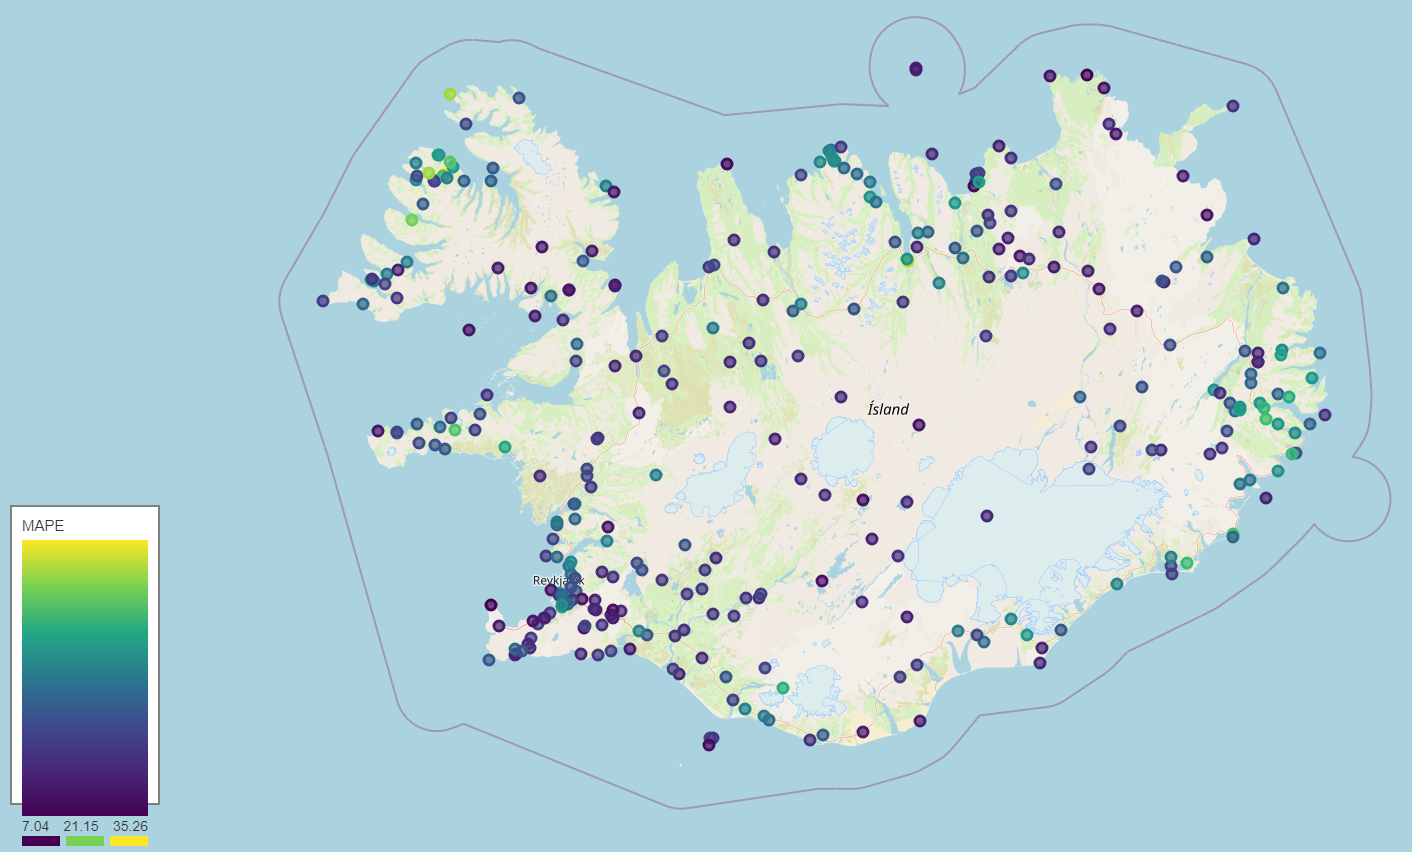
\includegraphics[scale = 0.5]{Figures/errorMap.png}
    \caption[MAPE error distribution of stations shown on a map of Iceland.]{The MAPE error of each station in data shown as color gradient circles. That is each station is represented by one circle, with the error value represented as a color gradient from dark blue to yellow. The lowest error at a single station was around 7\% at Garðskagaviti and the highest around 35\% at Seljalandsdalur. It is important to note that the model is trained using a cutoff of 10 m/s and this cutoff point is determined using the reanalysis wind at 15 meters above ground.}
    \label{fig:errorMap}
\end{figure}

\begin{table}[h]
    \caption[Model result looking at closed wind speed intervals]{The MAPE results for different AWSL intervals. Here instead of training for all data above a certain threshold put of the wind, training is done only on data between two wind speeds. The percentage variance in gust factor as a function of wind speed increases with decreasing wind speed. Measured wind speed is used for the cutoff and thus have data leakage. This results should thus be somewhat comparable to the last column in Table (\ref{table:results})}
    \label{table:closed_intervals}
    \centering
    \begin{tabular}{lcc}
        \toprule
        \textbf{Interval} &  \multicolumn{2}{c}{\textbf{MAPE}}\\
        $[m/s]$ & Without Elevation & With Elevation\\
        \midrule
        $[5, 10[$ & 17.2\% & 15.4\%\\ %10.6\%\\
        $[10, 15[$ & 14.1\% & 11.9\%\\ %7.8\%\\
        $[15, 20[$ & 13.2\% & 10.9\%\\ %6.4\%\\
        $[20, 25[$ & 14.9 \% & 11.6\%\\ %6.3\%\\
        $[25, 30[$ & 17.0\% & 16.0\%\\ %7.1\%\\
        \bottomrule
    \end{tabular}
\end{table}

Table (\ref{table:closed_intervals}) shows no improvement over the values in the last column in Table (\ref{table:results}). As previously mentioned, the gust factor decreases with increasing wind speed and thus, training on intervals and lessening this effect might be expected to give better results. This does not seem to be the case. Some interesting sites to look closer at for drivers might include places like Kjalarnes, Ingólfsfjall, Þrengsli and others. These can be seen in Table (\ref{table:specific_sites}).

\begin{table}[h]
    \caption[Model result by stations of interest]{The MAPE results of different stations for several stations of interest, both when training for the specific site and when the stations are a part of the general data. For every station the AWSL is set at 10 m/s. In training for a single station at a time, some site specific information can be gauged. This does not mean that the a better result can be reached for that site. Factors such as the number of datapoints at given location can significantly impact the result. This table uses the measured wind speed to determine the cut off for data points. This leads to some data leakage and an increased performance compared to using the reanalysis CARRA speed for cut off.}
    \label{table:more_specific_sites}
    \centering
    \begin{tabular}{lcc}
        \toprule
        \textbf{Station name} & \multicolumn{2}{c}{\textbf{MAPE}}\\
         & Baseline & Model\\
        \midrule
        Fáskrúðsfjörður & 28.2\% & 21.8\%\\
        Ingólfsfjall & 30.0\% & 19.6\%\\
        Kjalarnes & 20.7\% & 13.5\% \\
        Sandskeið & 13.0\% & 10.2\%\\
        Seyðisfjörður & 32.1\% & 23.0\%\\
        Þjórsárdalur & 12.2\% & 11.4\%\\
        Þrengsli & 13.6\% & 11.3\%\\
        \bottomrule
    \end{tabular}
\end{table}

\begin{figure}[h]
    \centering
    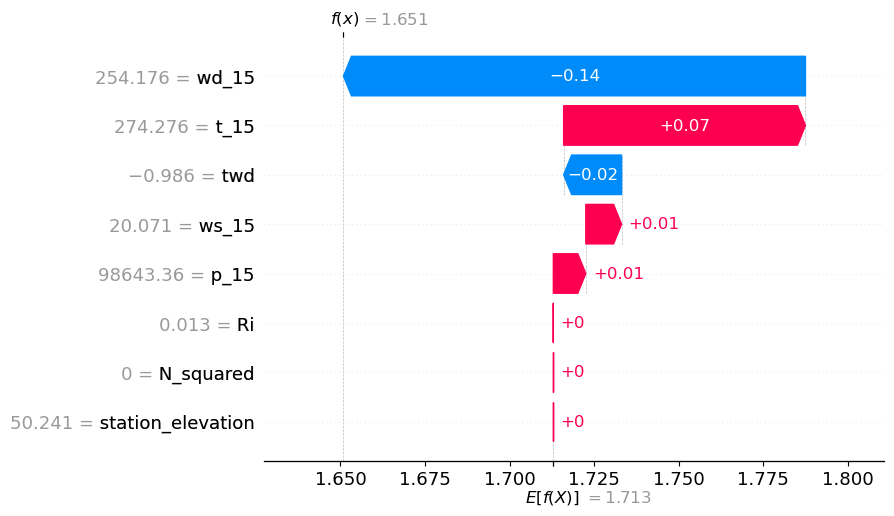
\includegraphics[scale = 0.6]{Figures/shap_plots/waterfall_plot.png}
    \caption[Feature importance for a single observation of a neural network.]{Feature importance of a neural network with model architecture as described in Table \ref{table:gridSearchHyperparamters} and data as described in Table \ref{table:trainDataExample}. In this specific instance the wind direction ($wd_{15}$) has the highest negative influence and the temperature has the highest positive influence. Elevation data is excluded when working with Shapley values, as the contribution of each elevation point is very low and there are very many of them. To see their influence on the model output see Table \ref{table:results}.}
    \label{fig:ShapleyWaterfall}
\end{figure}

In Figure (\ref{fig:ShapleySummary}) the contribution of each feature, excluding the elevation points, can be seen for the model in general (a significant subset of data is used). Looking at Figure (\ref{fig:ShapleySummary}), there is an outlier. Exactly calculating the Shapley values is time intensive, in the subset shown there is an outlier that skews the figure and makes it so that viewing the importance distribution excluding the outlier is difficult. For this reason, another shapley summary vas created that looked at different, and larger distribution. This can be seen in Figure (\ref{fig:ShapleySummary2}).

\begin{figure}
    \centering
    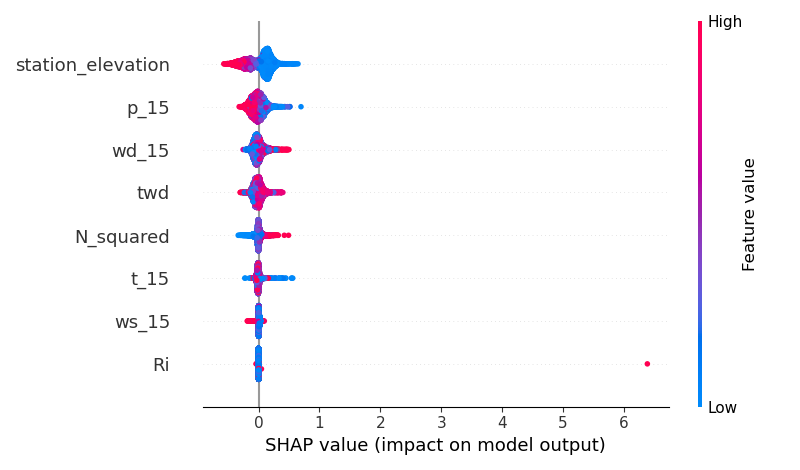
\includegraphics[scale = 0.6]{Figures/shap_plots/summary_plot.png}
    \caption[Summary feature importance of a neural network.]{Feature importance of a neural network with model architecture as described in Table \ref{table:gridSearchHyperparamters} and data as described in Table \ref{table:trainDataExample}. We can see that generally multiple factors influence the prediction, with the station elevation being highly influential. There is seemingly one outlier for the Richardson number, which usually has very little influence. Elevation data is excluded when working with Shapley values, as the contribution of each elevation point is very low and there are very many of them. To see their influence on the model output see Table \ref{table:results}.}
    \label{fig:ShapleySummary}
\end{figure}

\begin{figure}
    \centering
    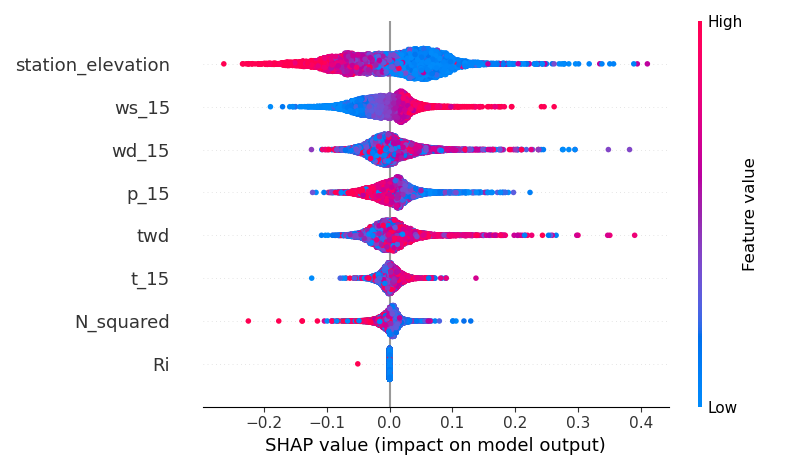
\includegraphics[scale = 0.6]{Figures/shap_plots/summary_plot_190924_.png}
    \caption[Summary feature importance of a neural network using a larger distribution of data.]{Feature importance of a neural network with model architecture as described in Table \ref{table:gridSearchHyperparamters} and data as described in Table \ref{table:trainDataExample}. Generally multiple factors influence the prediction, with the station elevation being highly influential. Elevation data is excluded when working with Shapley values, as the contribution of each elevation. In contrast to Figure (\ref{fig:ShapleySummary}), the distribution doesn't have as extreme outliers. This means that more details can be seen in the figure. The X-axis shows the influence of feature values on the model. The color gradient shows the value of each feature. As an example, there is a very red value for station elevation (top line, all the way to the left). This means that in this instance, the station elevation contributed around -0.25 to the final output and that the station had an elevation significantly above average.}
    \label{fig:ShapleySummary2}
\end{figure}

The Figures (\ref{fig:ShapleySummary}) and (\ref{fig:ShapleySummary2}) show the summary for a model trained only on the features shown and not on landscape elevation of the surrounding area. This is done as the number of points there is too high to display in one figure (70 total points). Looking specifically at Figure (\ref{fig:ShapleySummary2}), the station elevation is most influential and the Richardson number's influence is very low. Most of the feature values bunch up in the middle, while the station elevation is elongated compared to other features. Station elevation seems to have two bunches on either side of 0. Overall, the values seem to be skewed to the right of 0. This would be expected as the predicted values are expected to be in the range of 1.2-2, or at least always above 1 by definition. Finally, for the Shapley values, looking that all the data there are again outliers that skew the data so that spotting general distribution is difficult. This can be seen in Figure (\ref{fig:ShapleySummary3}).

\begin{figure}
    \centering
    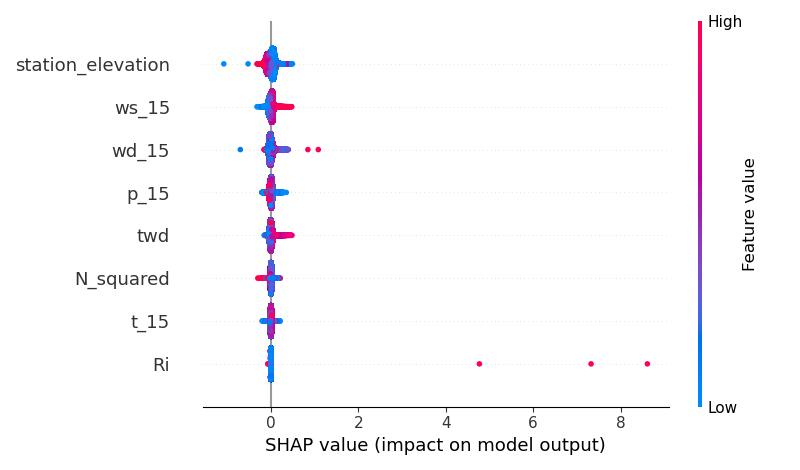
\includegraphics[scale = 0.6]{Figures/shap_plots/summary_plot_190924_full_10ms.png}
    \caption[Summary feature importance of a neural network using entire dataset.]{Feature importance of a neural network with model architecture as described in Table \ref{table:gridSearchHyperparamters} and data as described in Table \ref{table:trainDataExample}. The distribution seems to be the same as before, discounting the outliers.}
    \label{fig:ShapleySummary3}
\end{figure}

These plots can also be done by looking at individual stations. The model is then trained on all examples and afterwards the summary plot created using only points for each station. Stations of interest include stations listed in Table \ref{table:specific_sites}. These plots can all be seen in Figures (\ref{fig:ShapleySummaryAkrafjall} - \ref{fig:ShapleySummaryKeflavikurflugvollur}).

\begin{figure}
    \centering
    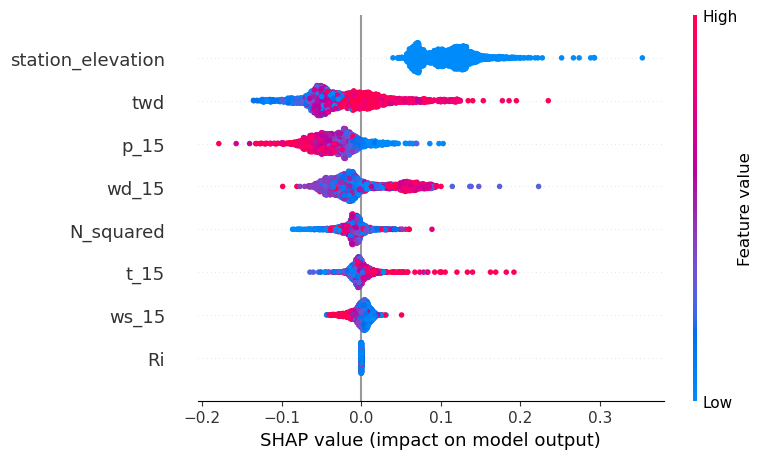
\includegraphics[scale = 0.6]{Figures/shap_plots/summary_plot_31572.png}
    \caption[Summary feature importance of a neural network only looking at AWS at Akrafjall.]{Feature importance of a neural network with model architecture as described in Table \ref{table:gridSearchHyperparamters} and data as described in Table \ref{table:trainDataExample}. This plot only looks at datapoints from Akrafjall. This seems to show the same distribution as previous summary plots. Station elevation is influential and Richardson number has no impact.}
    \label{fig:ShapleySummaryAkrafjall}
\end{figure}

\begin{figure}
    \centering
    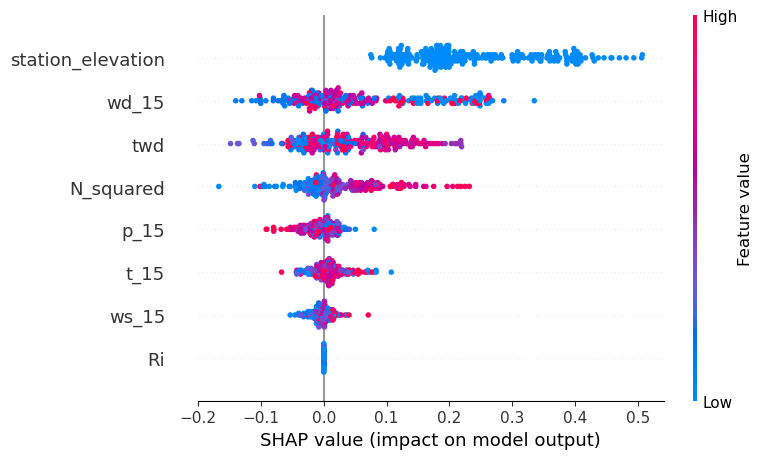
\includegraphics[scale = 0.6]{Figures/shap_plots/summary_plot_35553.png}
    \caption[Summary feature importance of a neural network only looking at AWS at Almannaskarð.]{Feature importance of a neural network with model architecture as described in Table \ref{table:gridSearchHyperparamters} and data as described in Table \ref{table:trainDataExample}. This plot only looks at datapoints from Almannaskarð. This seems to show the same distribution as previous summary plots. Station elevation is influential and Richardson number has no impact.}
    \label{fig:ShapleySummaryAlmannaskarð}
\end{figure}

\begin{figure}
    \centering
    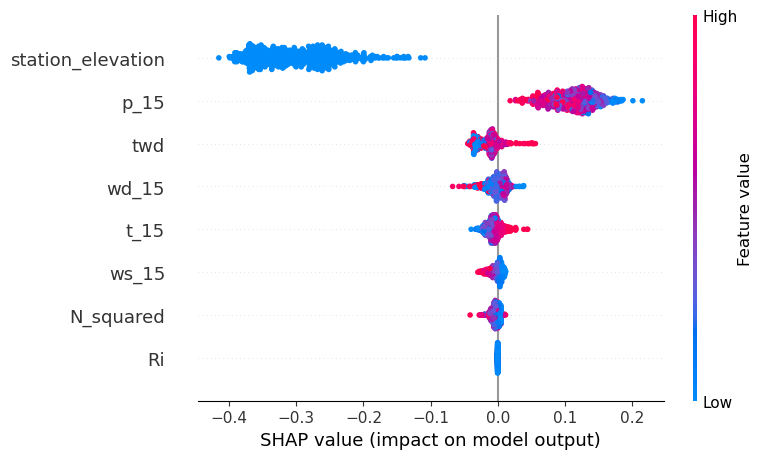
\includegraphics[scale = 0.6]{Figures/shap_plots/summary_plot_6745.png}
    \caption[Summary feature importance of a neural network only looking at AWS at Ásgarðsfjall.]{Feature importance of a neural network with model architecture as described in Table \ref{table:gridSearchHyperparamters} and data as described in Table \ref{table:trainDataExample}. This plot only looks at datapoints from Ásgarðsfjall. This seems to show the same distribution as previous summary plots. Station elevation is influential and Richardson number has no impact.}
    \label{fig:ShapleySummaryAsgarðsfjall}
\end{figure}

\begin{figure}
    \centering
    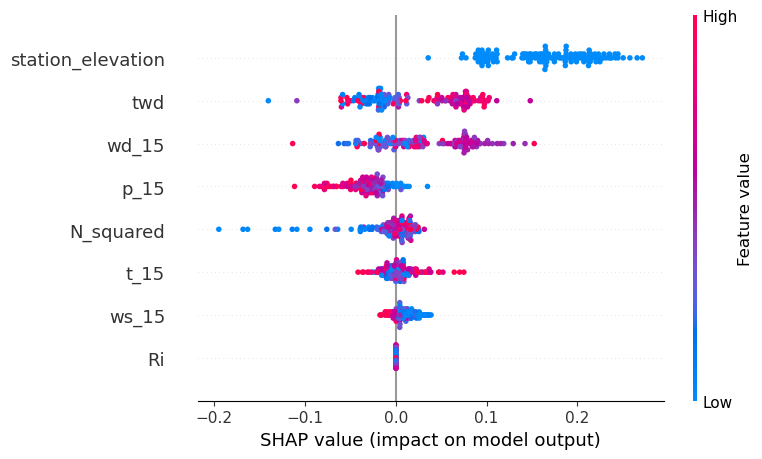
\includegraphics[scale = 0.6]{Figures/shap_plots/summary_plot_1470.png}
    \caption[Summary feature importance of a neural network only looking at AWS at Háahlíð.]{Feature importance of a neural network with model architecture as described in Table \ref{table:gridSearchHyperparamters} and data as described in Table \ref{table:trainDataExample}. This plot only looks at datapoints from Háahlíð. This seems to show the same distribution as previous summary plots. Station elevation is influential and Richardson number has no impact.}
    \label{fig:ShapleySummaryHaahlid}
\end{figure}

\begin{figure}
    \centering
    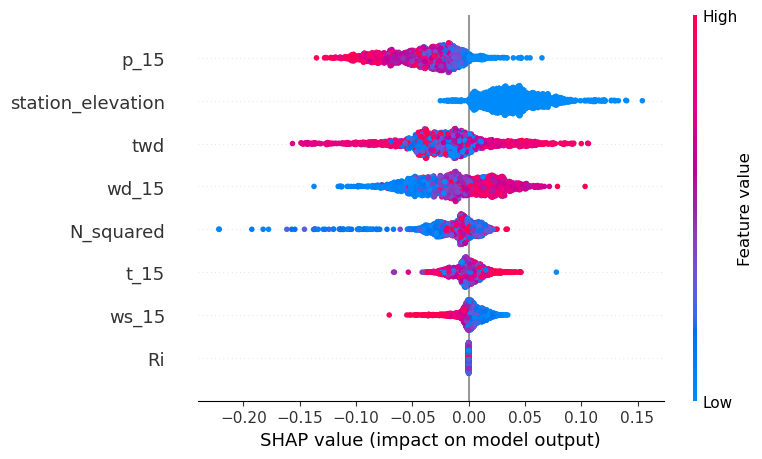
\includegraphics[scale = 0.6]{Figures/shap_plots/summary_plot_1350.png}
    \caption[Summary feature importance of a neural network only looking at AWS at Keflavíkurflugvöllur.]{Feature importance of a neural network with model architecture as described in Table \ref{table:gridSearchHyperparamters} and data as described in Table \ref{table:trainDataExample}. This plot only looks at datapoints from Keflavíkurflugvöllur. This seems to show the same distribution as previous summary plots. Station elevation is influential and Richardson number has no impact.}
    \label{fig:ShapleySummaryKeflavikurflugvollur}
\end{figure}

In each of these plots, even without the feature labels, the station elevation is easily noticed as the value is constant for a station. This is not noteworthy. What is noteworthy is the range of impact from this single value. For simpler models, this would not happen. It is important to note that SHAP assumes feature independece\cite{Salih_2024}. This might explain why the impact of the Richardson number is so low. Both the squared Brunt–Väisälä frequency and the Richardson number are derived features from reanalysis data. They carry with them some extra information over the other features in the dataset. This is because both are variables over elevation ranges. That is, as seen in Equations (\ref{eqn:Ri}, \ref{eqn:N}), both are dependent on values at lower and upper elevations and try to describe the stability of that range. Shapley tries to assign contribution values for each feature for each observation. SHAP assumes that the features are independent, but this is not the case. It is clearly not the case for the derived variables, but how the contribution should be distributed between the features is not clear. Seemingly the SHAP python package is giving all the impact to the Brunt–Väisälä squared frequency and none to Richardson number. If the Brunt–Väisälä would be excluded from the data, the impact of the Richardson number would likely increase. Another point to note is that the features are ordered by their impact. This means that the station elevation is the most impactful for each plot, but the ordering of other variables changes. Looking at Figure (\ref{fig:ShapleySummary3}), which shows the Shapley summary plot for all data, the wind speed is the second most important feature. This is reversed in Figure (\ref{fig:ShapleySummaryAkrafjall}). This is not unexpected as Akrafjall station was specifically selected as the MAE for reanalysis wind speed was very high as can be seen in Table (\ref{fig:ShapleySummaryAkrafjall}), where you will also find the stations whose summary plot is shown in Figures (\ref{fig:ShapleySummaryAlmannaskarð}, \ref{fig:ShapleySummaryAsgarðsfjall}) and these also fall into the category of very high MAE for wind speed. What is interesting is that the reanalysis wind speed is also of low impact at stations like Háahlíð and Keflavíkurflugvöllur, as shown in Figures (\ref{fig:ShapleySummaryHaahlid}, \ref{fig:ShapleySummaryKeflavikurflugvollur}). These stations had the lowest of MAE for difference between measured wind speed and reanalysis wind speed. As the summary plot over all stations (Figure (\ref{fig:ShapleySummary3})) shows that reanalysis wind speed is impactful, might lead to the conclusion that the reanalysis wind speed is not a good predictor at these locations or something else is skewing the data. A simpler way to look at feature importance is to create models that are trained on and use to predict different sets of parameters. The results of such a comparison can be seen in Table \ref{table:setsOfParams}.

\begin{table}[h]
    \caption[Model results for different sets of parameters.]{...}
    \label{table:setsOfParams}
    \centering
    \begin{tabular}{lc}
        \toprule
        \textbf{Model parameters} & \textbf{MAPE}\\
        \midrule
        Baseline constant & 23.9\%\\
        $ws_{15}$ & 17.2\%\\
        $[ws_{15}, t_{15}, p_{15}, wd_{15}]$ & 16.7\% \\
        $[ws_{15}, t_{15}, p_{15}, wd_{15}, ASL, twd]$ & 13.8\% \\
        $[ws_{15}, t_{15}, p_{15}, wd_{15}, ASL, twd, N, Ri]$ & ---\\
        $[ws_{15}, t_{15}, p_{15}, wd_{15}, ASL, twd, N, Ri]$ + DEM & ---\\
        $[ws_{15,250,500}, t_{15,250,500}, p_{15,250,500}, wd_{15,250,500}, ASL, twd, N, Ri]$ & --- \\
        \bottomrule
    \end{tabular}
\end{table}

\end{document}
